%definira klasu dokumenta 
\documentclass[12pt]{report} 

%prostor izmedu naredbi \documentclass i \begin{document} se zove uvod. U njemu se nalaze naredbe koje se odnose na cijeli dokument

%osnovni LaTex ne može riješiti sve probleme, pa se koriste različiti paketi koji olakšavaju izradu željenog dokumenta
\usepackage[croatian]{babel} 
\usepackage{amssymb}
\usepackage{amsmath}
\usepackage{txfonts}
\usepackage{mathdots}
\usepackage{titlesec}
\usepackage{array}
\usepackage{lastpage}
\usepackage{etoolbox}
\usepackage{tabularray}
\usepackage{color, colortbl}
\usepackage{adjustbox}
\usepackage{geometry}
\usepackage[classicReIm]{kpfonts}
\usepackage{hyperref}
\usepackage{fancyhdr}
\usepackage{graphicx}
\usepackage{color}

\definecolor{dkgreen}{rgb}{0,0.6,0}
\definecolor{gray}{rgb}{0.5,0.5,0.5}
\definecolor{mauve}{rgb}{0.58,0,0.82}
\usepackage{listings}
\lstset{frame=tb,
	language=Java,
	aboveskip=3mm,
	belowskip=3mm,
	showstringspaces=false,
	columns=flexible,
	basicstyle={\small\ttfamily},
	numbers=none,
	numberstyle=\tiny\color{gray},
	keywordstyle=\color{blue},
	commentstyle=\color{dkgreen},
	stringstyle=\color{mauve},
	breaklines=true,
	breakatwhitespace=true,
	tabsize=3
}


\usepackage{float}
\usepackage{setspace}
\restylefloat{table}


\patchcmd{\chapter}{\thispagestyle{plain}}{\thispagestyle{fancy}}{}{} %redefiniranje stila stranice u paketu fancyhdr

%oblik naslova poglavlja
\titleformat{\chapter}{\normalfont\huge\bfseries}{\thechapter.}{20pt}{\Huge}
\titlespacing{\chapter}{0pt}{0pt}{40pt}


\linespread{1.3} %razmak između redaka

\geometry{a4paper, left=1in, top=1in,}  %oblik stranice

\hypersetup{ colorlinks, citecolor=black, filecolor=black, linkcolor=black,	urlcolor=black }   %izgled poveznice


%prored smanjen između redaka u nabrajanjima i popisima
\newenvironment{packed_enum}{
	\begin{enumerate}
		\setlength{\itemsep}{0pt}
		\setlength{\parskip}{0pt}
		\setlength{\parsep}{0pt}
	}{\end{enumerate}}

\newenvironment{packed_item}{
	\begin{itemize}
		\setlength{\itemsep}{0pt}
		\setlength{\parskip}{0pt}
		\setlength{\parsep}{0pt}
	}{\end{itemize}}




%boja za privatni i udaljeni kljuc u tablicama
\definecolor{LightBlue}{rgb}{0.9,0.9,1}
\definecolor{LightGreen}{rgb}{0.9,1,0.9}

%Promjena teksta za dugačke tablice
\DefTblrTemplate{contfoot-text}{normal}{Nastavljeno na idućoj stranici}
\SetTblrTemplate{contfoot-text}{normal}
\DefTblrTemplate{conthead-text}{normal}{(Nastavljeno)}
\SetTblrTemplate{conthead-text}{normal}
\DefTblrTemplate{middlehead,lasthead}{normal}{Nastavljeno od prethodne stranice}
\SetTblrTemplate{middlehead,lasthead}{normal}

%podesavanje zaglavlja i podnožja

\pagestyle{fancy}
\lhead{Programsko inženjerstvo}
\rhead{IS2-Digitalizacija}
\lfoot{Septabil}
\cfoot{stranica \thepage/\pageref{LastPage}}
\rfoot{\today}
\renewcommand{\headrulewidth}{0.2pt}
\renewcommand{\footrulewidth}{0.2pt}


\begin{document} 
	
	
	
	\begin{titlepage}
		\begin{center}
			\vspace*{\stretch{1.0}} %u kombinaciji s ostalim \vspace naredbama definira razmak između redaka teksta
			\LARGE Programsko inženjerstvo\\
			\large Ak. god. 2021./2022.\\
			
			\vspace*{\stretch{3.0}}
			
			\huge $IS2-Digitalizacija$\\
			\Large Dokumentacija, Rev. \textit{2}\\
			
			\vspace*{\stretch{12.0}}
			\normalsize
			Grupa: \textit{$Septabil$}\\
			Voditelj: \textit{Dominik Jurinčić}\\
			
			
			\vspace*{\stretch{1.0}}
			Datum predaje: \textit{14. 01. 2022.}\\
	
			\vspace*{\stretch{4.0}}
			
			Nastavnik: \textit{Igor Stančin}\\
		
		\end{center}

	
	\end{titlepage}

	
	\tableofcontents


	\chapter{Dnevnik promjena dokumentacije}
		
		\textbf{\textit{Kontinuirano osvježavanje}}\\
				
		
	\begin{longtblr}[
		label=none
		]{
			width = \textwidth, 
			colspec={|X[2]|X[13]|X[3]|X[3]|}, 
			rowhead = 1
		}
		\hline
		\textbf{Rev.}    & \textbf{Opis promjene/dodatka} & \textbf{Autori} & \textbf{Datum}\\[3pt] \hline
		0.1 & Dodani osnovni elementi arhitekture sustava i baze podataka.    & Dominik Jurinčić, Borna Radojčić i Ivan Lovrić & 14.11.2021.         \\[3pt] \hline 
		0.2    & Dodane manje modifikacije na modelu baze podataka. & Borna Radojčić i Ivan Lovrić & 14.11.2021.     \\[3pt] \hline 
		0.3 & Dodan dio općeg opisa projektnog zadatka. & Marko Bunić & 14.11.2021. \\[3pt] \hline 
		0.4 & Promjene na dokumentaciji baze podataka, ostalih zahtjeva i vremena rada na projektu.  & Borna Radojčić i Ivan Lovrić & 17.11.2021. \\[3pt] \hline 
		0.5 & Ispravljen dio dokumentacije vezan uz arhitekturu sustava.  & Dominik Jurinčić & 17.11.2021. \\[3pt] \hline 
		0.6 & Dodan dijagram obrazaca uporabe. & Filip Martinović & 17.11.2021. \\[3pt] \hline 
		0.7 & Postavljena cjelovita planirana baza podataka, pripadni relacijski dijagram i sekvencijski dijagrami.& Borna Radojčić, Ivan Lovrić i Jakov Prister&19.11.2021. \\[3pt] \hline 
		0.8 & Dovršen opis projektnog zadatka. & Marko Bunić & 19.11.2021. \\[3pt] \hline 
		0.9 & Promijenjeni ostali zahtjevi, dodan dnevnik sastajanja i izbrisani nebitni dijelovi. & Marko Bunić i Dominik Jurinčić & 19.11.2021. \\[3pt] \hline 
		0.10 & Dodani dijagrami razreda. & Filip Martinović & 19.11.2021. \\[3pt] \hline
		\textbf{1.0} & Verzija samo s bitnim dijelovima za 1. ciklus & * & 19.11.2021. \\[3pt] \hline
		1.1 & Popravljen dio dokumentacije vezan uz opću arhitekturu sustava. & Dominik Jurinčić & 7.1.2022. \\[3pt] \hline
		1.2 & Ispravljeni sekvencijski dijagrami. & Jakov Prister i Borna Radojčić & 10.1.2022. \\[3pt] \hline
		1.3 & Dodane upute za puštanje u pogon. & Borna Radojčić & 11.1.2022. \\[3pt] \hline
		1.4 & Dodane dijagram razreda. & Filip Martinović & 12.1.2022. \\[3pt] \hline
		1.5 & Dodan unaprijeđeni ER dijagram. & Ivan Lovrić i Borna Radojčić & 13.1.2022. \\[3pt] \hline
		1.6 & Dodani dijagrami aktivnosti i razmještaja. & Jakov Prister & 14.1.2022. \\[3pt] \hline
		1.7 & Dodane korištene tehnologije i alati. & Dominik Jurinčić & 14.1.2022. \\[3pt] \hline
		1.8 & Dodan dijagram komponenti. & Ivan Lovrić & 14.1.2022. \\[3pt] \hline
		1.9 & Dodan dijagram stanja. & Marko Bunić & 14.1.2022. \\[3pt] \hline
		1.10 & Dodan zaključak. & Marko Bunić i Ivan Lovrić & 14.1.2022. \\[3pt] \hline
		\textbf{2.0} & Potpuna dokumentacija. & * & 14.1.2022. \\[3pt] \hline
		
	\end{longtblr}
	
	
	
	\chapter{Opis projektnog zadatka}
		
		\textbf{\textit{dio 1. revizije}}\\
		
	
		
		
	
		
		
		Cilj ovog projekta je razviti prikladnu strukturu i programsku podršku za stvaranje mobilne aplikacije "DigiFyl".
		Aplikacija će biti dostupna i prikladna za korištenje svim računovodstvenim tvrtkama koje žele prijeći na novi i moderniji način skladištenja svojih dokumenata te im omogućiti brz i jednostavan prijelaz.
		U današnjem dobu gdje je digitalizacija sve jači faktor u svim granama proizvodnje i osobnog života, sustavi koji se njome ne koriste su zastarjeli. Još jedna značajna pozitivna strana korištenja DigiFyl digitaliziranog sustava skladištenja dokumenta je što se smanjuje potreban fizički međuljudski kontakt, što uvelike olakšava rad s dokumentima u današnje vrijeme. Također je i dijeljenje i traženje određenih dokumenata jednostavnije i efikasnije nego rad s fizičkim dokumentima.
		
		Naše usluge se dijele na aplikaciju koju će svi korisnici unutar klijentske tvrtke koristiti na svojem mobitelu i pozadinsku strukturu koja će podržavati dio funkcionalnosti aplikacije i skladištiti te čuvati dokumente tvrtke. Cilj nam je učiniti potrebne promjene pri prijelazu na korištenje naših usluga vrlo jednostavnim za korisničku tvrtku, učiniti sam prijelaz brzim i efikasnim te napraviti aplikaciju jednostavnom i intuitivnom za korištenje. Glavne funkcionalnosti aplikacije su skeniranje tekstualnih dokumenata u fizičkom obliku pomoću kamere te kreiranje njegove digitalne kopije koju je moguće dijeliti s drugim korisnicima i skladištiti u sustavu. Također je unutar aplikacije implementiran i korisnički sustav koji podržava rad unutar tvrtke.
		
		
		\medskip
		\textbf{Pokazni primjer funkcionalnosti aplikacije, korisnici i tipovi dokumenata}
		\medskip
		
		
		 Pri prvom pokretanju aplikacije korisnika, korisniku se na izbor otvara mogućnost kreacije novog računa ili prijavljivanja na vlastiti račun. Pri kreaciji novog računa, korisnik bira i svoju ulogu na temelju koje mu aplikacija kasnije nudi različite funkcionalnosti i dodjeljuje prava. Za kreaciju novog računa potrebni su:
				
		\begin{packed_item}
			
			\item  korisničko ime
			\item  lozinka
			\item  ime i prezime
			\item  broj mobitela
			\item  email adresa
			\item  uloga u tvrtki	
			
		\end{packed_item}
	
		Registracijom u sustav korisniku se dodjeljuju prava i funkcionalnosti izabrane uloge te korisnik šalje zahtjev za pristupanje zajednici određene tvrtke. Direktor tvrtke nakon kreacije računa kreira i tvrtku te on pregledava zahtjeve korisnika za pridruživanje tvrtki i odobrava ili odbija te iste zahtjeve. Također direktor može dodijeliti ta ista prava zaposlenicima koje odabere.
		
		\medskip
		\textbf{Uloge i njihove pripadne funkcionalnosti i prava su:}
		
			\begin{packed_item}
		\item\underbar{Zaposlenik}- su najbrojnija pozicija, njihova uloga je skeniranje dokumenata i slanje skeniranih dokumenata revizoru. Zaposlenik također može vidjeti povijest svojih skeniranja. 
		
		\item\underbar{Revizor}- ima iste funkcije i prava kao i korisnik, uz dodatna prava i funkcije. Dodatna funkcija je da nakon što revizor skenira dokument, aplikacija automatski određuje tip dokumenta i računovođu kojem se skenirani dokument šalje. Također revizor pregledava sve pristigle dokumente i šalje ih odgovarajućim računovođama.
		
		\item\underbar{Računovođa}- dobivene dokumente arhivira u bazu podataka. Također, računovođa
		 ima opciju slanja dokumenta direktoru na potpis prije arhiviranja te arhiviranja nakon potpisa. 
		
		\item\underbar{Direktor}- uz funkcije i prava svih ostalih korisnika, može i vidjeti povijest svih dokumenta te povijest i
		statistike svih zaposlenika, kreira tvrtku pri kreiranja računa, prihvaća ili odbija zahtjeve korisnika svojoj tvrtki te može mijenjati pozicije svoj zaposlenika i dodjeljivati im određena prava, kao pravo prihvaćanja zahtjeva tvrtki.
		\end{packed_item}
	
	\medskip
	\textbf{Tipovi dokumenata}
	
		\begin{packed_item}
			
			
			\item\underbar{računi} Računi će unutar dokumenta na kraju teksta imati oznaku  računa koja je veliko slovo R te šest znamenaka. Računi osim oznake sadrže ime klijenta, artikle s cijenama i ukupnu cijenu
			\item\underbar{ponude} ponude će unutar dokumenta na kraju teksta imati veliko slovo P i devet znamenaka. Ponude će osim oznake sadržavati artikle s cijenama i ukupnu cijenu
			\item\underbar{interni dokumenti} Interni dokumenti će unutar dokumenta na kraju teksta imati „INT“ i četiri znamenke. Ostatak internog dokumenta je nestrukturirani tekst.
			
		\end{packed_item}
	
		\medskip
		\textbf{Pregled elastičnosti infrastrukture aplikacije i poslovnog modela}
			\\
		Naša aplikacija i sustav pokriva osim predstavljene aplikacije, i pozadinski kod, i bazu podataka
			unutar koje bi se čuvali svi spremljeni dokumenti. Budući da smo za našu serversku stranu odabrali servise Amazon Web Services-a, to nam daje mogućnost održati našu pozadinsku strukturu skalabilnom koja nam uvelike olakšava dio posla s predviđanjem potrebnog razmjera pozadinske strukture i omogućava lako i okretno prilagođavanje potrebama naših klijenata. Zato na samom početku, naš sustav ima male zahtjeve unutar Amazonovog Web Clouda te naše potrebe ne izlaze izvan dozvoljenih granica bez plaćanja AWS-ovih usluga što nam je sasvim dovoljno za testiranje našeg proizvoda od strane klijenata. Nakon što bi se određeni klijent odlučio za korištenje naših usluga i predstavio nam svoje potrebe, mi bi prikladno odredili potreban razmjer našeg pozadinskog sistema, naknadu koju bi plaćali AWS-u za traženo proširenje usluga, i uzimajući sve u obzir, predstavili klijentu cijenu naših usluga među koje ulazi i podrška korisnicima naših usluga. Predstavljen način izdavanja ponuda klijentima i prikladnog mijenjanja sustava naknadno je mnogo efikasniji i jednostavniji radi brzih i jednostavnih mogućnosti mijenjanja skale pozadinskog sustava koju AWS pruža. Nadalje, nakon prikladnog širenja sustava za jednog klijenta, dolazak i korištenje naših usluga novog klijenta nikako neće utjecati na prethodnog klijenta. Promjene i povećanja sustava imaju i više opcija te, uz prethodno navedena svojstva, mi jednostavno možemo odrediti prikladno rješenje, odrediti zahtjeve novog proširenog sustava unutar AWS-ovog web clouda. Znajući troškove korištenja AWS-ovih usluga, lako možemo predstaviti novom klijentu ponudu korištenja naših usluga koja nikako utječe na ostale klijente. Time korištenje naših usluga od strane klijenata je jednostavno, nikakve integracije sustava nisu potrebne jer se mi brinemo o samoj strukturi koja čuva i skladišti dokumente korisnika te je naš sustav prilagodljiv i okretan za sve potrebne promjene i nove zahtjeve.
		
		\medskip
		\textbf{Pregled prilagodljivosti korisničkog sustava}
			\\
		Pri ponudi naših usluga novoj korisničkoj stranci, također nudimo i kreaciju posebno prilagođenog sustava korisnika dizajniranom isključivo za tu korisničku stranku. Uzimajući u obzir tipove dokumenata, različite pozicije pojedinih zaposlenika unutar tvrtke i njihovih ovlasti i funkcija, pomoću naših postojećih predložaka sustava korisnika i dokumenata zajedno s izradom i implementacijom svega novog potrebnog za specifični zahtjev, brzo i jednostavno kreiramo prilagođen sustav korisnika, dokumenata i funkcionalnosti. Cijena ove usluge ovisi o samim specifikacijama određenog zahtjeva.
		


		
		\medskip
		\textbf{Usporedba s konkurentnim proizvodima na tržištu}
			\\
		Na tržištu već postoje mnoge aplikacije slične našoj po tome što implementiraju optičko prepoznavanje znakova i omogućuju skeniranje tekstualnih zapisa sa slike te prebacivanje skeniranog teksta u druge formate. Primjeri takvih aplikacija su Text Scanner i Text Fairy dostupne na Google Play-u. Isto tako, mnogi pružatelji usluga skladištenja i rada s digitaliziranim dokumentima su već duže vremena dostupni na tržištu, kao što su ClearDATA i FileCloud, te postoje i mnogi koji uz digitalno skladištenje dokumenta pružaju i usluge skeniranja dokumenata kao što su Apyxx Technologies i GRM Document Management.
			
		Ono po čemu se naša aplikacija razlikuje od navedenih je što osim što sadrži potpunu pozadinsku potporu za skladištenje i rad sa skeniranim tekstualnim dokumentima zajedno s odgovarajućim korisničkim sistemom i održavanjem cijelog sistema dokumenata, također nudi elastičnost i prilagodljivost svakoj zasebnoj korisničkoj stranci u obliku prilagođavanja korisničkog sistema i skale pozadinskog sustava. Korištenje naše aplikacije je jednostavno i intuitivno te dolazi uz kontinuiranu korisničku podršku. Time su naše usluga najbolji izbor za izradu digitalnih kopija dokumenata, održavanje njihovog sistema skladištenja i rad među korisnicima sa digitaliziranim dokumentima za odgovarajuće tvrtke kojima su potrebne navedene usluge.
		
		
		
		
		
		\eject
		
		
		
	
	\chapter{Specifikacija programske potpore}
		
	\section{Funkcionalni zahtjevi}
	
	\textbf{\textit{dio 1. revizije}}\\
	
	
	
	
	\noindent \textbf{Dionici:}
	
	\begin{packed_enum}
		
		\item Zaposlenici\begin{packed_enum}
			\item Revizor			
			\item Računovođa
			\item Normalan zaposlenik
		\end{packed_enum}
		
		\item Direktor
		\item Razvojni tim
		
		
	\end{packed_enum}
	
	\noindent \textbf{Aktori i njihovi funkcionalni zahtjevi:}
	
	
	\begin{packed_enum}
		\item  \underbar{Neregistrirani/neprijavljeni korisnik (inicijator) moze::}
		
		\begin{packed_enum}
			
			\item pristupiti Login aktivnosti
			\item pristupiti Sign-up aktivnosti
			
		\end{packed_enum}
		
		\item  \underbar{Radnik može:}
		
		\begin{packed_enum}
			
			\item pristupiti Login aktivnosti i prijaviti se
			\item skenirati dokument i podvrti točnost skeniranja ili označiti dokument kao krivo skeniran
			\item pogledati svoju povijest skeniranja
			
		\end{packed_enum}
		
		\item  \underbar{Računovođa može:}
		
		\begin{packed_enum}
			
			\item pristupiti Login aktivnosti i prijaviti se
			\item skenirati dokument i podvrti točnost skeniranja ili označiti dokument kao krivo skeniran
			\item pogledati svoju povijest skeniranja
			\item arhivirati dokument
			\item poslati dokument direktoru na potpis
			\item arhivirati potpisani dokument
			\item dobiti pregled dokumenta prije slanja na potpis / arhiviranja 
			
		\end{packed_enum}
		
		\item  \underbar{Revizor može:}
		
		\begin{packed_enum}
			
			\item pristupiti Login aktivnosti i prijaviti se
			\item skenirati dokument i podvrti točnost skeniranja ili označiti dokument kao krivo skeniran
			\item pogledati svoju povijest skeniranja
			\item provjeriti dokument i preusmijeriti ga računovođi koji je zadužen za taj tip dokumenta
			\item dobiti pregled dokumenta prije slanja na preusmjerivanja
			
			
			
		\end{packed_enum}
		
		\item  \underbar{Direktor može:}
		
		\begin{packed_enum}
			
			\item pristupiti Login aktivnosti i prijaviti se
			\item skenirati dokument i podvrti točnost skeniranja ili označiti dokument kao krivo skeniran
			\item pogledati svoju povijest skeniranja
			\item vidjeti statistike radnika firme
			\item potpisati dokument
			\item dobiti pregled dokumenta prije slanja na preusmjerivanja
			
		\end{packed_enum}
		\item  \underbar{Baza podataka:}
		
		\begin{packed_enum}
			
			\item pohranjuje sve podatke o korisnicima i njihovim ovlastima
			\item pohranjuje skenirane dokumente i ispavnost njihovog skeniranja
			
			
		\end{packed_enum}
		
		
	\end{packed_enum}
	
	\eject 
	
	
	
	\subsection{Obrasci uporabe}
	
	\textbf{\textit{dio 1. revizije}}
	
	\subsubsection{Opis obrazaca uporabe}

	
	
	\noindent \underbar{\textbf{UC1 - Login}}
	\begin{packed_item}
		
		\item \textbf{Glavni sudionik: }Korisnik aplikacije
		\item  \textbf{Cilj:} prijaviti se u aplikaciju
		\item  \textbf{Sudionici:} Baza podataka
		\item  \textbf{Preduvjet:} Korisnik je dobio password i username od direktora
		\item  \textbf{Opis osnovnog tijeka:}
		
		\item[] \begin{packed_enum}
			
			\item Korisnik aplikacije unosi username i password u to predviđena "text input-a"
			\item pritišće Login gumb
			\item biva preusmjeren na određenu aktivnost, ovisno o svojoj ulozi unatar firme
			
		\end{packed_enum}
		
		\item  \textbf{Opis mogućih odstupanja:}
		
		\item[] \begin{packed_item}
			
			\item[1.a] Unos krivih podataka
			\item[] \begin{packed_enum}
				
				\item Ponoviti unos, te paziti prilikom unosa podataka
				\item Provjeriti s direktorom ispravnost podataka
				
			\end{packed_enum}
			
			
		\end{packed_item}
	\end{packed_item}
	
	\noindent \underbar{\textbf{UC2 - Skreniranje dokumenta}}
	\begin{packed_item}
		
		\item \textbf{Glavni sudionik: }Korisnik aplikacije
		\item  \textbf{Cilj:} Skrenirati dokument
		\item  \textbf{Sudionici:} Baza podataka, Revizor
		\item  \textbf{Preduvjet:} Korisnik je prijavljen
		\item  \textbf{Opis osnovnog tijeka:}
		
		\item[] \begin{packed_enum}
			
			\item Korisnik aplikacije pritišće gumb za odabir skeniranja dokumenta
			\item Smiruje mobilni uređaj kako skeniranje ne bi bilo mutno
			\item Fokusira kameru
			\item Pritišće gumb za skeniranje, to jest slikanje dokumenta
			\item Korisnik odabire je li dokument ispravno skeniran
			\item Ako je dokument skreniran od strane zaposlenika i obilježen kao ispravno skeniran, taj dokument se šalje revizoru
			\item Ako revizor skenira dokument onda se dokument šalje računovođi koji je zadužen za tu vrstu dokumenta
			
			
		\end{packed_enum}
		
		\item  \textbf{Opis mogućih odstupanja:}
		
		\item[] \begin{packed_item}
			
			\item[2.a] Mutna slika
			\item[] \begin{packed_enum}
				
				\item Pokušati držati mobilni uređaj mirno pri skeniranju
				
				
			\end{packed_enum}
			
			\item[5.a] Neispravno skeniran dokoment
			\item[] \begin{packed_enum}
				
				\item Skenirati dokument ponovo
				
				
			\end{packed_enum}
			
			
		\end{packed_item}
	\end{packed_item}
	
	
	
	\noindent \underbar{\textbf{UC3 - Preusmjeravanje dokumenta računovođi}}
	\begin{packed_item}
		
		\item \textbf{Glavni sudionik: }Revizor
		\item  \textbf{Cilj:} Preusmjeriti podatke
		\item  \textbf{Sudionici:} Baza podataka, Računovođa
		\item  \textbf{Preduvjet:} Revizor je prijavljen i ima dokument koji može preusmjeriti
		\item  \textbf{Opis osnovnog tijeka:}
		
		\item[] \begin{packed_enum}
			
			\item Revizor pritišće gumb za 
			pregled "dobro" skeniranih dokumenata
			\item Potvrđuje da je dokument dobro skeniran pritiskom na taj dokument
			\item Odabirom ispravnog dokumenta može ga poslati računovođi koji je zadužen za taj dokument prtiskom gumba "pošalji računovođi" i odabirom računovođe
			
			
		\end{packed_enum}		
	\end{packed_item}
	
	
	
	\noindent \underbar{\textbf{UC4 - Arhiviranje dokumenta}}
	\begin{packed_item}
		
		\item \textbf{Glavni sudionik: }Računovođa
		\item  \textbf{Cilj:} Arhivirati ispravno skenirani dokument
		\item  \textbf{Sudionici:} Baza podataka
		\item  \textbf{Preduvjet:} Računovođa je prijavljen i ima dokument koji može arhivirati
		\item  \textbf{Opis osnovnog tijeka:}
		
		\item[] \begin{packed_enum}
			
			\item Računovođa pritišće gumb za 
			pregled potencijalno potpisanih i preusmjerenih dokumenata
			\item Računovođa pritiskom na dokument označuje dokument za arhiviranje ili slanje na potpis
			\item Utvrđuje da je dokument ispravno preusmjeren ili potpisan, te pritišće gumb "Arhiviraj"
			\item Dokumentu dobiva oznaku "arhiviran" u bazi podataka
			
			
			
		\end{packed_enum}		
	\end{packed_item}
	
	\noindent \underbar{\textbf{UC5 - Slanje dokumenta direktoru na potpis}}
	\begin{packed_item}
		
		\item \textbf{Glavni sudionik: }Računovođa
		\item  \textbf{Cilj:} Poslati dokument direktoru na potpis
		\item  \textbf{Sudionici:} Baza podataka, direktor
		\item  \textbf{Preduvjet:} Računovođa je prijavljen i ima dokument koji može poslati direktoru
		\item  \textbf{Opis osnovnog tijeka:}
		
		\item[] \begin{packed_enum}
			
			\item Računovođa pritišće gumb za 
			pregled potencijalno potpisanih i preusmjerenih dokumenata
			\item Računovođa odabire ne-potpisan dokument i šalje ga direktoru na potpis pritiskom gumba "pošalji na potpis"
			
			
			
		\end{packed_enum}		
	\end{packed_item}
	
	\noindent \underbar{\textbf{UC6 - Potpis dokumenta}}
	\begin{packed_item}
		
		\item \textbf{Glavni sudionik: }Direktor
		\item  \textbf{Cilj:} Potpisati dokument
		\item  \textbf{Sudionici:} Baza podataka
		\item  \textbf{Preduvjet:} Direktor je prijavljen i ima dokument koji može potpisati
		\item  \textbf{Opis osnovnog tijeka:}
		
		\item[] \begin{packed_enum}
			
			\item Direktor pritišće gumb "Dokumenti za potpis" za 
			pregled preusmjerenih dokumenata
			\item Direktor odabire jedan ili više ne-potpisanih dokumenta i potpisuje ih pritiskom gumba "Potpiši"
			\item Dokument se sprema u bazu podataka kao potpisan dokument
			
			
		\end{packed_enum}		
	\end{packed_item}
	
	\noindent \underbar{\textbf{UC7 - Pregled povijesti dokumenata}}
	\begin{packed_item}
		
		\item \textbf{Glavni sudionik: }Direktor
		\item  \textbf{Cilj:} Pregledati povijest dokumenata
		\item  \textbf{Sudionici:} Baza podataka, direktor
		\item  \textbf{Preduvjet:} Direktor je prijavljen i baza podataka ima barem jedan dokument
		\item  \textbf{Opis osnovnog tijeka:}
		
		\item[] \begin{packed_enum}
			
			\item Direktor pritišće gumb za 
			pregled povijest i statisiku
			\item Direktor pritišće gumb za pregled skeniranih dokumenata
			
			
		\end{packed_enum}		
	\end{packed_item}
	
	\noindent \underbar{\textbf{UC8 - Pregled statistike  zaposlenika}}
	\begin{packed_item}
		
		\item \textbf{Glavni sudionik: }Direktor
		\item  \textbf{Cilj:} Pregledati statistike zaposlenika
		\item  \textbf{Sudionici:} Baza podataka, direktor
		\item  \textbf{Preduvjet:} Direktor je prijavljen i postoji barem jedan zaposlenik
		\item  \textbf{Opis osnovnog tijeka:}
		
		\item[] \begin{packed_enum}
			
			\item Direktor pritišće gumb za 
			pregled povijest i statisiku
			\item Direktor pritišće gumb za pregled statistike radnika
			
			
			
			
		\end{packed_enum}	
		\item  \textbf{Opis mogućih odstupanja:}
		
		\item[] \begin{packed_item}
			
			\item[2.a] Ne-prikaz nekih statistika
			\item[] \begin{packed_enum}
				
				\item Ako se neke statistike ne prikažu, to znači da korisnik nema ovlasti za te radnje
			\end{packed_enum}	
		\end{packed_item}
	\end{packed_item}
	
	
	
	\noindent \underbar{\textbf{UC9 - Stvaranje korisnika}}
	\begin{packed_item}
		
		\item \textbf{Glavni sudionik: }Direktor
		\item  \textbf{Cilj:} Stvoriti korisnika
		\item  \textbf{Sudionici:} Baza podataka, korsinik
		\item  \textbf{Preduvjet:} Direktor je prijavljen
		\item  \textbf{Opis osnovnog tijeka:}
		
		\item[] \begin{packed_enum}
			
			\item Korisnik pritišće gumb "sign up" za 
			Signup aktivnost
			\item Korisnik upisuje podatke na za to predviđena mjesta
			\item Korisnik pritišće gumb "Signup"
			\item Korisnik biva pohranjen u bazu podataka
			
			
		\end{packed_enum}		
	\end{packed_item}
				
					
				\subsubsection{Dijagrami obrazaca uporabe}
					
				
					
				
			\subsection{Sekvencijski dijagrami}
			\subsubsection{Login korisnika}
			
			Korisnik unosi korisničko ime i lozinku te se pokušava ulogirati u aplikaciju. Uneseni podaci se preko API Gatewaya i lambda funkcije šalju u bazu podataka. Tamo se provjerava postoji li korisnik s unesenim korisničkim imenom, ako ne postoji korisniku su ispisuje poruka LoginInvalid. Ako je baza pronašla korisnika provjerava njegovu šifru u bazi podataka s upisanom šifrom i ako se one podudaraju ispisuje korisniku LoginValid, u suprotnom ispisuje LoginInvalid.
			\eject
			
			\begin{figure}
				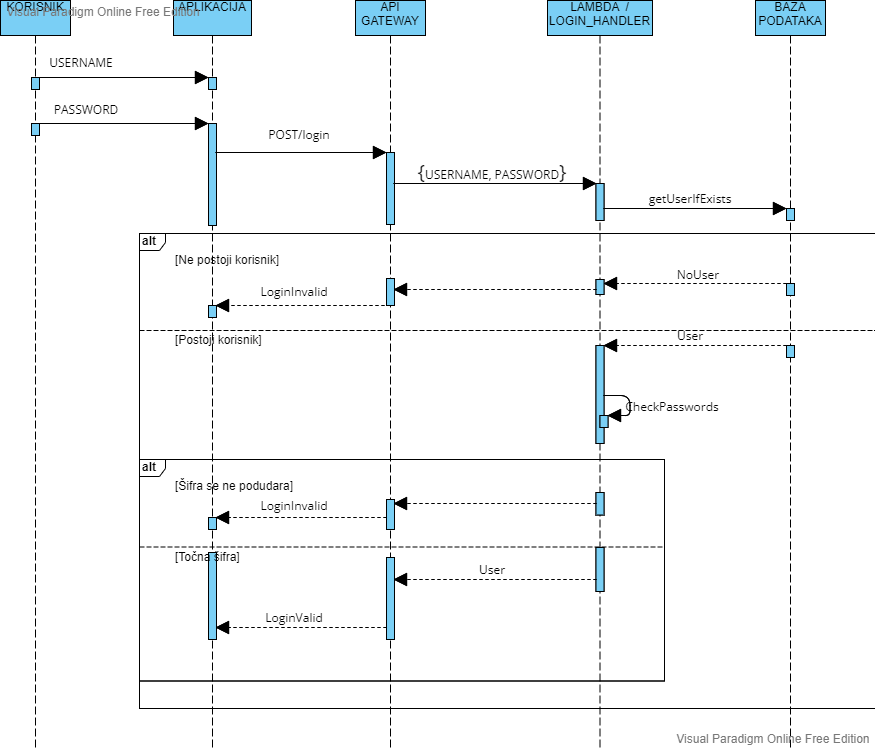
\includegraphics[width=\linewidth]{./dijagrami/Login.png}
				\caption{Sekvencijski dijagram za login}
				\label{fig:Login}
			\end{figure}
			
			
			
			\subsubsection{Registracija korisnika}
			
			Korisnik unosi korisničko ime, ime, prezime, lozinku i poziciju. Uneseni se podaci preko API Gatewaya i lambda funkcije šalju u bazu podataka. Tamo se provjerava postoji li već korisnik s navedenim korisničkim imenom, ako da ispisuje LoginInvalid. U suprotnom slučaju unosi korisnika u bazu podataka i ispisuje LoginValid.
			\eject
			
			\begin{figure}
				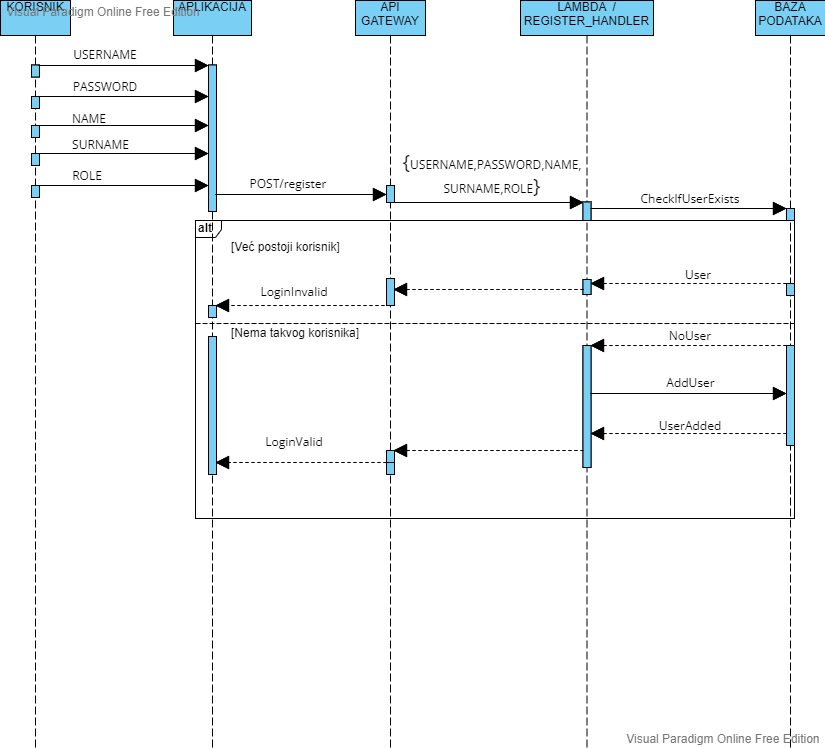
\includegraphics[width=\linewidth]{./dijagrami/Register.png}
				\caption{Sekvencijski dijagram za registraciju}
				\label{fig:Register}
			\end{figure}
			\subsubsection{OCR funkcija}
			
			Korisnik skenira željeni dokument te u aplikaciji poziva funkciju OCR koja mu vraća sažetak dokumenta. Zatim korisnik odlučuje točnost dokumenta te to označi u aplikaciji. Sažetak dokumenta i točnost se šalju u bazu podataka neovisno o korisnikovom odabiru.
			\eject
			
			\begin{figure}
				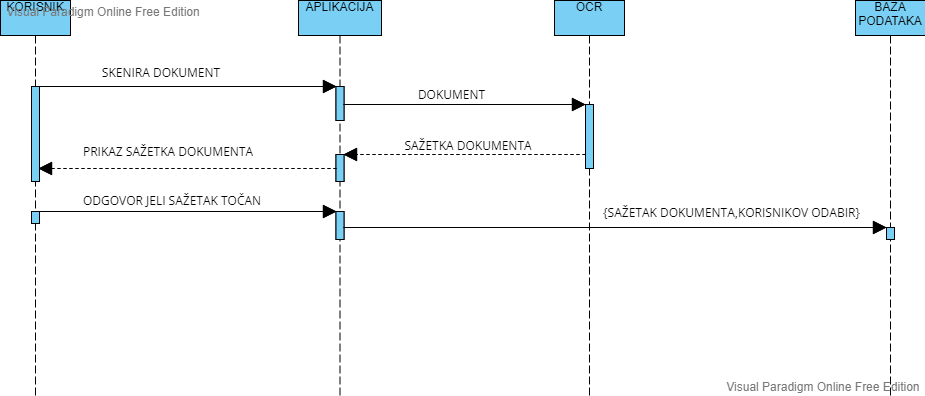
\includegraphics[width=\linewidth]{./dijagrami/OCR.png}
				\caption{OCR funkcija}
				\label{fig:OCR}
			\end{figure}
			
			\subsubsection{Povijest svih skeniranih dokumenata zaposlenika}
			
			Zaposlenik u aplikaciji traži povijest svih svojih skeniranih dokumenata. Preko API Gatewaya i lambda funkcije u bazi podatak se provjerava postoji li uopće neki skenirani dokument od zaposlenika, ako ne ispisuje zaposleniku da je povijest skeniranja prazna. Ako već postoje skenirani dokumenti u bazi podataka, aplikacija ih daje na pregled zaposleniku.
			\eject
			
			\begin{figure}
				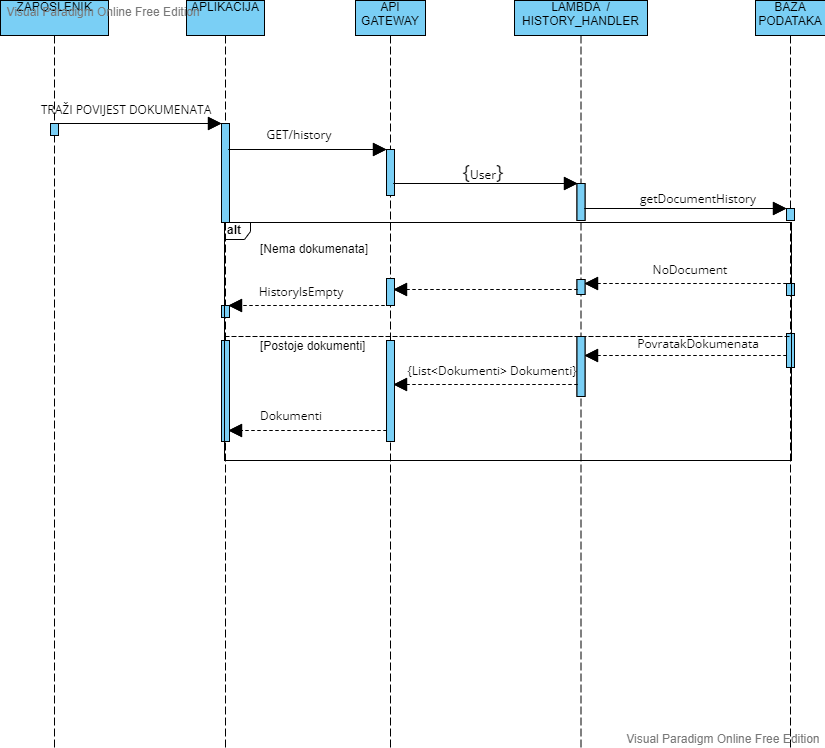
\includegraphics[width=\linewidth]{./dijagrami/History.png}
				\caption{Povijest svih skeniranih dokumenata zaposlenika}
				\label{fig:History}
			\end{figure}
			
		\section{Ostali zahtjevi}
		
			\textbf{\textit{dio 1. revizije}}\\
		 
			 
			 Podržani jezik našeg programskog sučelja je Engleski. Vrijeme odziva\\ aplikacije je gotovo trenutačno, možda oko pola sekunde čekanja između klika na login i ulaska u aplikaciju. Podržani broj korisnika nema gornje ograničenje, zato što uvijek možemo dodatno skalirati sustav. Trenutno koristimo AWS free tier usluge te imamo 20GB alociranog prostora i milijun besplatnih zahtjeva na AWS lambdu mjesečno. Sa rastom broja korisnika možemo po potrebi skalirati sustav po cijeni ponuđenoj od strane AWS-a. Podržana mobilna platforma je Android OS, aplikacija je pisana u Javi (Android Studiu) i Pythonu. Razina zaštite na\\ kompletnom sustavu je relativno niska, u bazu podataka se upisuje lozinka u\\ izvornom obliku, bez bilo kakve vrste kriptiranja. Jedina zaštita koju imamo je to što AWS, na kojem nam se sve nalazi, koristi https protokol. Aplikacija je jako pouzdana što se tiče registiranja korisnika i zapisa njihovih podataka u bazu podataka na AWS RDS poslužitelju te dohvaćanju tih podataka iz baze i validaciji prilikom prijave. Registracija je lagana i jednostavna, klikom na "\textit{signup}" gumb se mogu unijeti svi potrebni podaci, a korisničko ime i lozinka su kasnije potrebni za prijavu u sustav.
			 Korištenje aplikacije nakon prijave je isto jako jednostavno, sve opcije za svakog korisnika su ponuđene odmah na početnoj stranici aplikacije.
			 
			 
			 
	
	
\chapter{Arhitektura i dizajn sustava}
		 Arhitektura se može podijeliti na tri dijela:
	\begin{itemize}
		\item 	\textit{Frontend}
		\item 	\textit{Backend}
		\item 	\textit{Baza podataka}		
	\end{itemize}
		
		\underline{Frontend} predstavlja korisničko sučelje Android aplikacije i njegove funkcionalnosti. Korisničko sučelje prikazuje rezultate korisnikovih zahtjeva te olakšava njihovo slanje. Korisnik putem korisničkog sučelja šalje zahtjeve Backend-u. Korisnik može biti zaposlenik, revizor, računovođa ili direktor. Na temelju svoje uloge korisnici imaju različite ovlasti i samim time mogu slati različite zahtjeve.
		HTTP zahtjevi se šalju na Amazon AWS API Gateway koji je zadužen za obradu zahtjeva. API Gateway zatim prosljeđuje zahtjev backend-u.\\
		
		\underline{Backend} predstavlja dio programa koji se izvodi na web poslužitelju i omogućava izvršavanje zahtjeva koje korisnik šalje. Komunikacija Frontend-a i Backend-a odvija se HTTP protokolom. Nakon što Backend primi zahtjev koji je korisnik uputio, on iz njega izlučuje podatke potrebne za izvršavanje zahtjeva. Ti podaci nalaze se u body-ju HTTP zahtjeva. Backend je ostvaren korištenjem Amazon AWS Lambde. Za svaku vrstu zahtjeva stvorena je zasebna Lambda. Svaka Lambda sadrži funkciju koja kao argument prima body HTTP zahtjeva u obliku rječnika u kojem su ključevi nazivi parametara koji se se šalju zahtjevom. Zatim se izvrši kod funkcije i njena povratna vrijednost se ponovo šalje korisniku na frontend-u preko API Gateway-a. Funkcije u Lambdi koriste Psycopg2 adapter za slanje zahtjeva na bazu podataka. \\
		
		U \underline{bazi podataka} nalaze se podaci o korisnicima i dokumenti koje su skenirali. Baza je napravljena koristeci Amazon AWS RDS.\\\\\\
		
		Za izradu Frontend-a naše android aplikacije izabrali smo programski jezik Java, a za Backend smo koristili Python. Za razvoj Frontend-a koristili smo Android Studio, a za razvoj Backend-a Visual Studio Code razvojno okruženje.\\
	
		Raspodjela arhitekture na Frontend, Backend i bazu podataka omogućila je lakše ispitivanje pojedinih dijelova sustava kao i jednostavnije i nezavisnije razvijanje.
		
		
		\begin{figure}
			\centering
			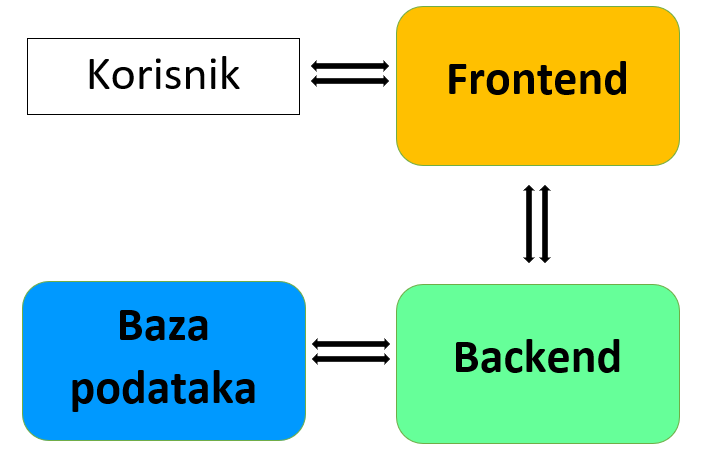
\includegraphics[scale=0.75]{./slike/Prikaz arhitekture.png}
			\caption{Arhitektura sustava}
			\label{fig:ARH}
		\end{figure}
		

		


		\section{Baza podataka}
			
			
			
		Koristili smo relacijsku bazu podataka koju smo napravili u postgreSQL-u.\\
		Trenutna početna verzija baze sadrži relaciju users.
		
			\subsection{Opis tablica}
			

			
				
				
				\begin{longtblr}[
					label=none,
					entry=none
					]{
						width = \textwidth,
						colspec={|X[8,l]|X[8, l]|X[20, l]|}, 
						rowhead = 1,
					} %definicija širine tablice, širine stupaca, poravnanje i broja redaka naslova tablice
					\hline \multicolumn{3}{|c|}{\textbf{users}}	 \\ \hline[3pt]
					\SetCell{LightGreen}userId & SERIAL	&  	Jedinstveni identifikator korisnika  	\\ \hline
					firstName	& VARCHAR(50) & Ime korisnika   	\\ \hline 
					lastName & VARCHAR(50) & Prezime korisnika   \\ \hline 
					username & VARCHAR(50)	& Korisničko ime korisnika - jedinstveno  		\\ \hline 
					userPswd & VARCHAR(50) & Lozinka korisnika  \\ \hline
					 userRole & VARCHAR(20) & Uloga korisnika   	\\ \hline 
				\end{longtblr}
				
			U tablici users zapisani su svi korisnici aplikacije, svaki korisnik ima jedinstveno korisničko ime (username) i dodjeljuje mu se jedinstveni identifikator (userId) koji je primarni ključ tablice.
			Ostali atributi koje svaki korisnik ima su njegovo ime i prezime, lozinka u aplikaciji (za prijavu mora unijeti korisničko ime i lozinku) i uloga unutar tvrtke.
			
			
					\begin{longtblr}[
					label=none,
					entry=none
					]{
						width = \textwidth,
						colspec={|X[8,l]|X[8, l]|X[20, l]|}, 
						rowhead = 1,
					} %definicija širine tablice, širine stupaca, poravnanje i broja redaka naslova tablice
					\hline \multicolumn{3}{|c|}{\textbf{scanHistory}}	 \\ \hline[3pt]
					\SetCell{LightGreen}docId & SERIAL &  Jedinstveni identifikator dokumenta  	\\ \hline
					\SetCell{LightBlue}userId & INT & Identifikator korisnika  	\\ \hline 
					scanDate & DATE & Datum skeniranja  \\ \hline 
				\end{longtblr}
			scanHistory je tablica koja u sebi sadrži sve skenirane dokumente, bili oni ispravno ili neispravno skenirani, ispravno skenirani dokumenti će otići u documents dok će neispravni samo ostati ovdje.
			Njeni atributi su docId (jedinstveni identifikator svakog skeniranog dokumenta), userId (jedinstveni identifikator korisnika koji je skenirao dokument) i datum skeniranja
			
				\begin{longtblr}[
				label=none,
				entry=none
				]{
					width = \textwidth,
					colspec={|X[8,l]|X[8, l]|X[20, l]|}, 
					rowhead = 1,
				} %definicija širine tablice, širine stupaca, poravnanje i broja redaka naslova tablice
				\hline \multicolumn{3}{|c|}{\textbf{documents}}	 \\ \hline[3pt]
				\SetCell{LightGreen}docId & INT	&  	Jedinstveni identifikator dokumenta  	\\ \hline
				docLabel & VARCHAR(10) & Oznaka dokumenta   	\\ \hline 
				docType & VARCHAR(1) & Tip dokumenta   	\\ \hline 
				docText & TEXT & Skenirani tekst   \\ \hline 
			\end{longtblr}
		Tablica documents sadrži podatke o svim dokumentima koji su potvrđeni kao ispravno skenirani, podaci koji su zapisani u njoj su docId (jedinstveni identifikator), docLabel (oznaka dokumenta), docType (tip dokumenta) i docText (skenirani tekst u dokumentu) 
		


\begin{longtblr}[
	label=none,
	entry=none
	]{
		width = \textwidth,
		colspec={|X[8,l]|X[8, l]|X[20, l]|}, 
		rowhead = 1,
	} %definicija širine tablice, širine stupaca, poravnanje i broja redaka naslova tablice
	\hline \multicolumn{3}{|c|}{\textbf{accountantResponsibility}}	 \\ \hline[3pt]
	\SetCell{LightGreen}userId & INT & Identifikator korisnika  	\\ \hline 
	responsibility & VARCHAR(1) & Zaduženje računovođe (Računi, ponude ili interni dokumenti)  \\ \hline 
	
\end{longtblr}

accountantResponsibility je tablica koja u sebi sadrži userId nekog računovođe i njegovo zaduženje (računi, ponude ili interni dokumenti)


\begin{longtblr}[
	label=none,
	entry=none
	]{
		width = \textwidth,
		colspec={|X[8,l]|X[8, l]|X[20, l]|}, 
		rowhead = 1,
	} %definicija širine tablice, širine stupaca, poravnanje i broja redaka naslova tablice
	\hline \multicolumn{3}{|c|}{\textbf{archive}}	 \\ \hline[3pt]
	\SetCell{LightGreen}archiveId & SERIAL &  Jedinstveni identifikator arhive  	\\ \hline
	\SetCell{LightBlue}docId & INT & Jedinstveni identifikator dokumenta  \\ \hline 
	\SetCell{LightBlue}userId & INT & Identifikator korisnika \\ \hline
	archivedDate & DATE & Datum arhiviranja \\ \hline
	signed & SMALLINT & Dokument potpisan/nepotpisan \\ \hline
	
\end{longtblr}

archive je tablica u koju se spremaju svi dokumenti koje računovođe arhiviraju,
svaka arhiva ima svoj jedinstveni identifikator (archiveId).
Atributi koji se spremaju uz archiveId su docId arhiviranog dokumenta, userId računovođe koji ga je arhivirao, datum arhiviranja i signed (dokument potpisan/ne)

\begin{longtblr}[
	label=none,
	entry=none
	]{
		width = \textwidth,
		colspec={|X[8,l]|X[8, l]|X[20, l]|}, 
		rowhead = 1,
	} %definicija širine tablice, širine stupaca, poravnanje i broja redaka naslova tablice
	\hline \multicolumn{3}{|c|}{\textbf{reviserPending}}	 \\ \hline[3pt]
	\SetCell{LightGreen}docId & INT &  Jedinstveni identifikator dokumenta  	\\ \hline
	\SetCell{LightBlue}userId & INT & Identifikator korisnika  	\\ \hline 
	
\end{longtblr}

reviserPending je tablica u koju se spremaju dokumenti koji se šalju revizoru, kad će revizor potvrđivati i proslijeđivati dokumente, pregledavati će dokumente iz ove tablice.
Ima samo 2 atributa, a to su docId dokumenta kojeg je zaposlenik poslao i userId revizora kojem se šalje taj dokument. 


\begin{longtblr}[
	label=none,
	entry=none
	]{
		width = \textwidth,
		colspec={|X[8,l]|X[8, l]|X[20, l]|}, 
		rowhead = 1,
	} %definicija širine tablice, širine stupaca, poravnanje i broja redaka naslova tablice
	\hline \multicolumn{3}{|c|}{\textbf{executivePending}}	 \\ \hline[3pt]
	\SetCell{LightGreen}docId & INT &  Jedinstveni identifikator dokumenta  	\\ \hline
	\SetCell{LightBlue}userId & INT & Identifikator korisnika  	\\ \hline 
	
\end{longtblr}

executivePending je tablica u koju se spremaju dokumenti koje računovođe šalju direktoru na potpis prije arhiviranja,
isto ima samo 2 atributa, a to su docId dokumenta poslanog na potpis i userId računovođe kojem se potpisani dokument treba vratiti. 


\begin{longtblr}[
	label=none,
	entry=none
	]{
		width = \textwidth,
		colspec={|X[8,l]|X[8, l]|X[20, l]|}, 
		rowhead = 1,
	} %definicija širine tablice, širine stupaca, poravnanje i broja redaka naslova tablice
	\hline \multicolumn{3}{|c|}{\textbf{accountantPending}}	 \\ \hline[3pt]
	\SetCell{LightGreen}docId & INT &  Jedinstveni identifikator dokumenta  	\\ \hline
	\SetCell{LightBlue}userId & INT & Identifikator korisnika  	\\ \hline 
	signaturePending & SMALLINT & Status potpisa  	\\ \hline 
	
\end{longtblr}

accountantPending je tablica u koju se spremaju dokumenti koji se šalju računovođi na arhiviranje.\\
Računovođa kojem će dokument biti dostavljen je odabran s obzirom na svoju odgovornost (tablica accountantResponsibility), atributi tablice accountantPending su docId dokumenta koji je poslan računovođi, userId računovođe kojem je poslan dokument i atribut signaturePending koji govori je li potpis tražen.\\
Ako je vrijednost atributa signaturePending 0, potpis nije tražen, ako je 1, potpis je tražen, ali direktor još nije potpisao dokument, a ako je 2, onda je potpis tražen i direktor je potpisao i vratio dokument. 




			
			\subsection{Dijagram baze podataka}
			
			\eject
			\begin{figure}
				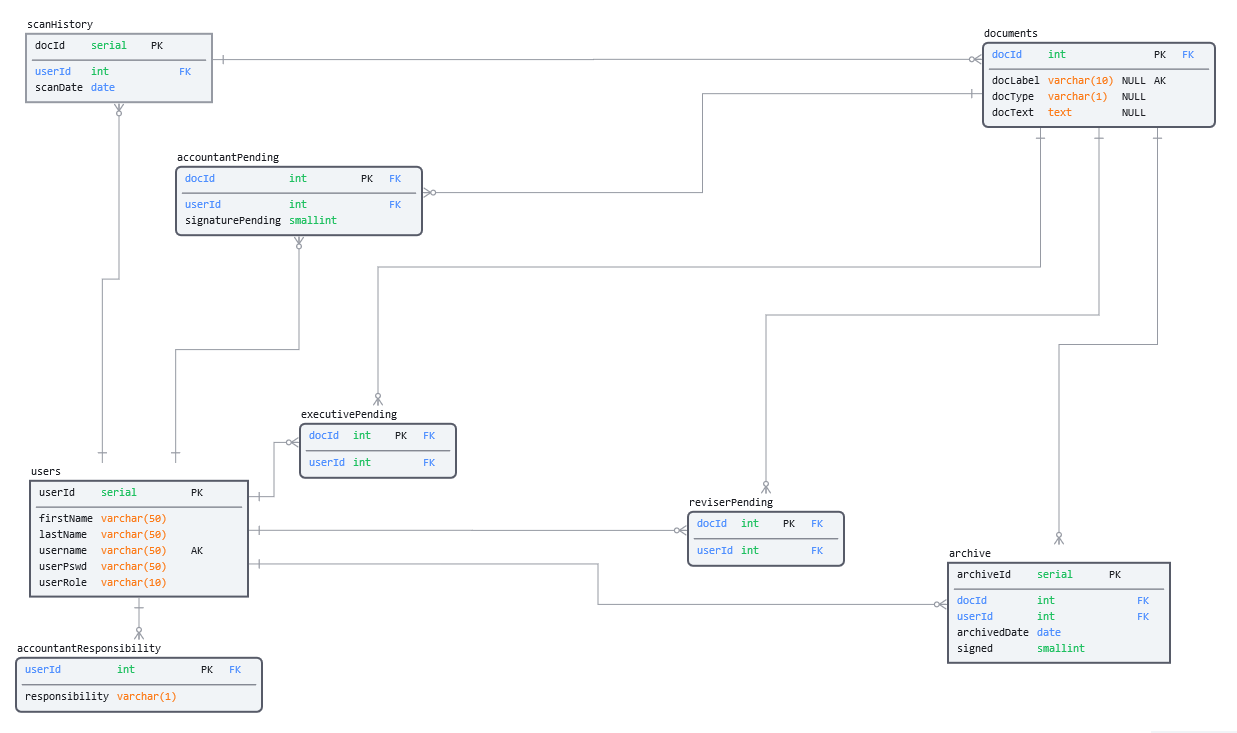
\includegraphics[width=\linewidth]{./dijagrami/ER.png}
				\caption{ER Diagram}
				\label{fig:ER}
			\end{figure}
			
			
		\section{Dijagram razreda}
			
			Na slici su prikazani razredi koji pripadaju backend dijelu MVC
			arhitekture.\\
			U izvornom kodu postoje samo razredi \textit{User} i \textit{Document}.\\ Razred \textit{User} ima atribut \textit{role} koji određuje kojim funkcijama "handlerima" instanca razreda ima pristup. Postoje tri tipa računovođa koji imaju pristup istim funkcijama. Jedina je razlika u tipu dokumenta kojega arhiviraju.\\
			Razred \textit{Document} ima atribut \textit{type} koji određuje tip dokumenta, te kojem računovođi se šalju. Svi tipovi imaju pristup jednakim funkcijama "handlerima".\\
			Različiti atributi \textit{role} i \textit{type} su u dijagramu prikazani kao razredi izvedeni iz razreda \textit{User} radi preglednosti.\\
			
			\begin{figure}
				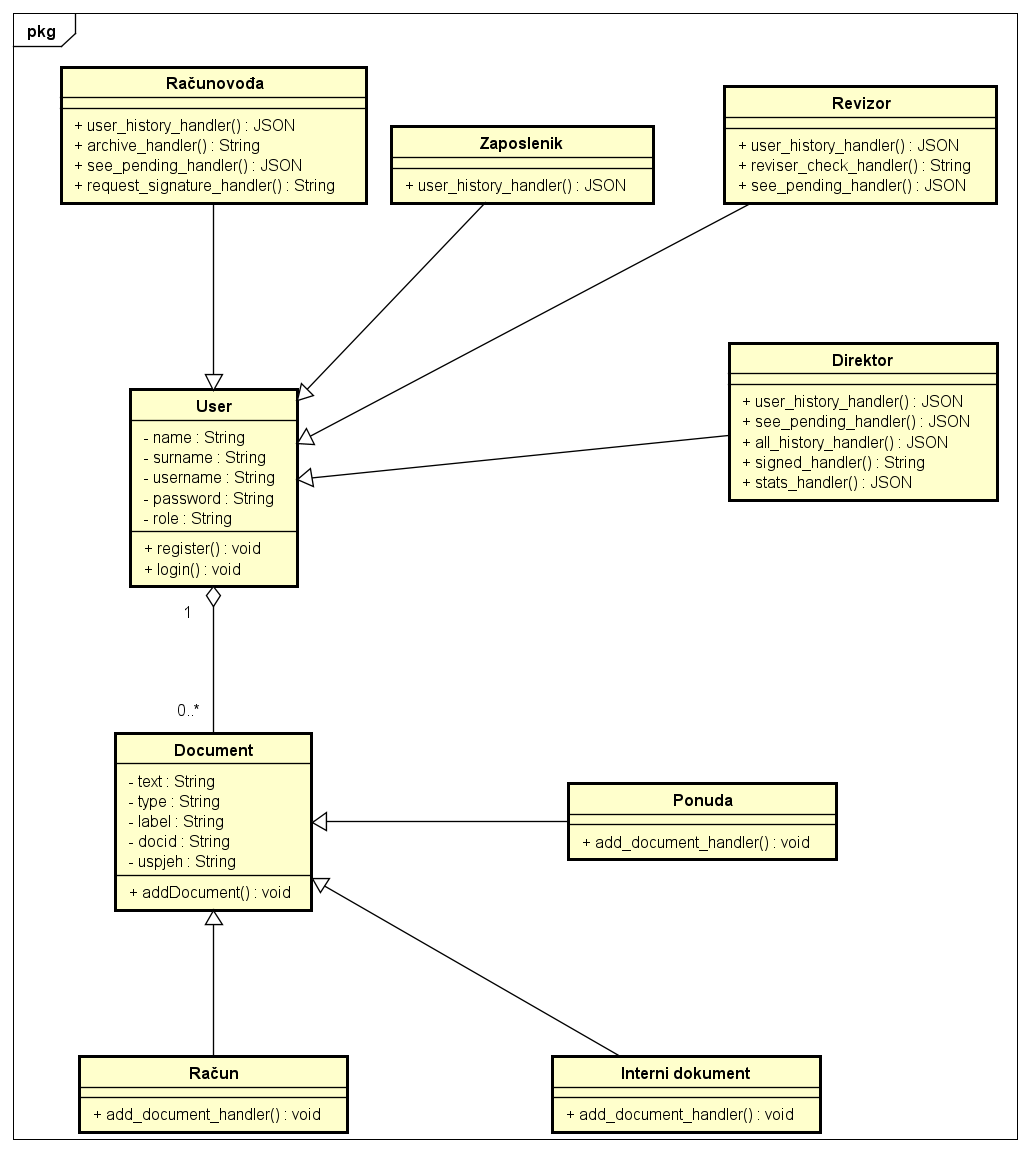
\includegraphics[width=\linewidth]{./dijagrami/dijagram_razreda.png}
				\caption{Dijagram razreda}
				\label{fig:Class}
			\end{figure}
			
			
			
			\eject
		
		\section{Dijagram stanja}
			
			
		
			
			U nastavku je dijagram stanja koji prikazuje stanja, odnosno "stranice" aplikacije. 
			Također su i naznačeni trenutci  u kojima aplikacija komunicira s back-endom. Uvedena je simplifikacija glavne aktivnosti zaposlenika, revizora, direktora i računovođe u glavnu aktivnost radi jednostavnijeg prikaza.
			
			\bigskip
			\bigskip
			\bigskip
			
			\begin{figure}[H]
				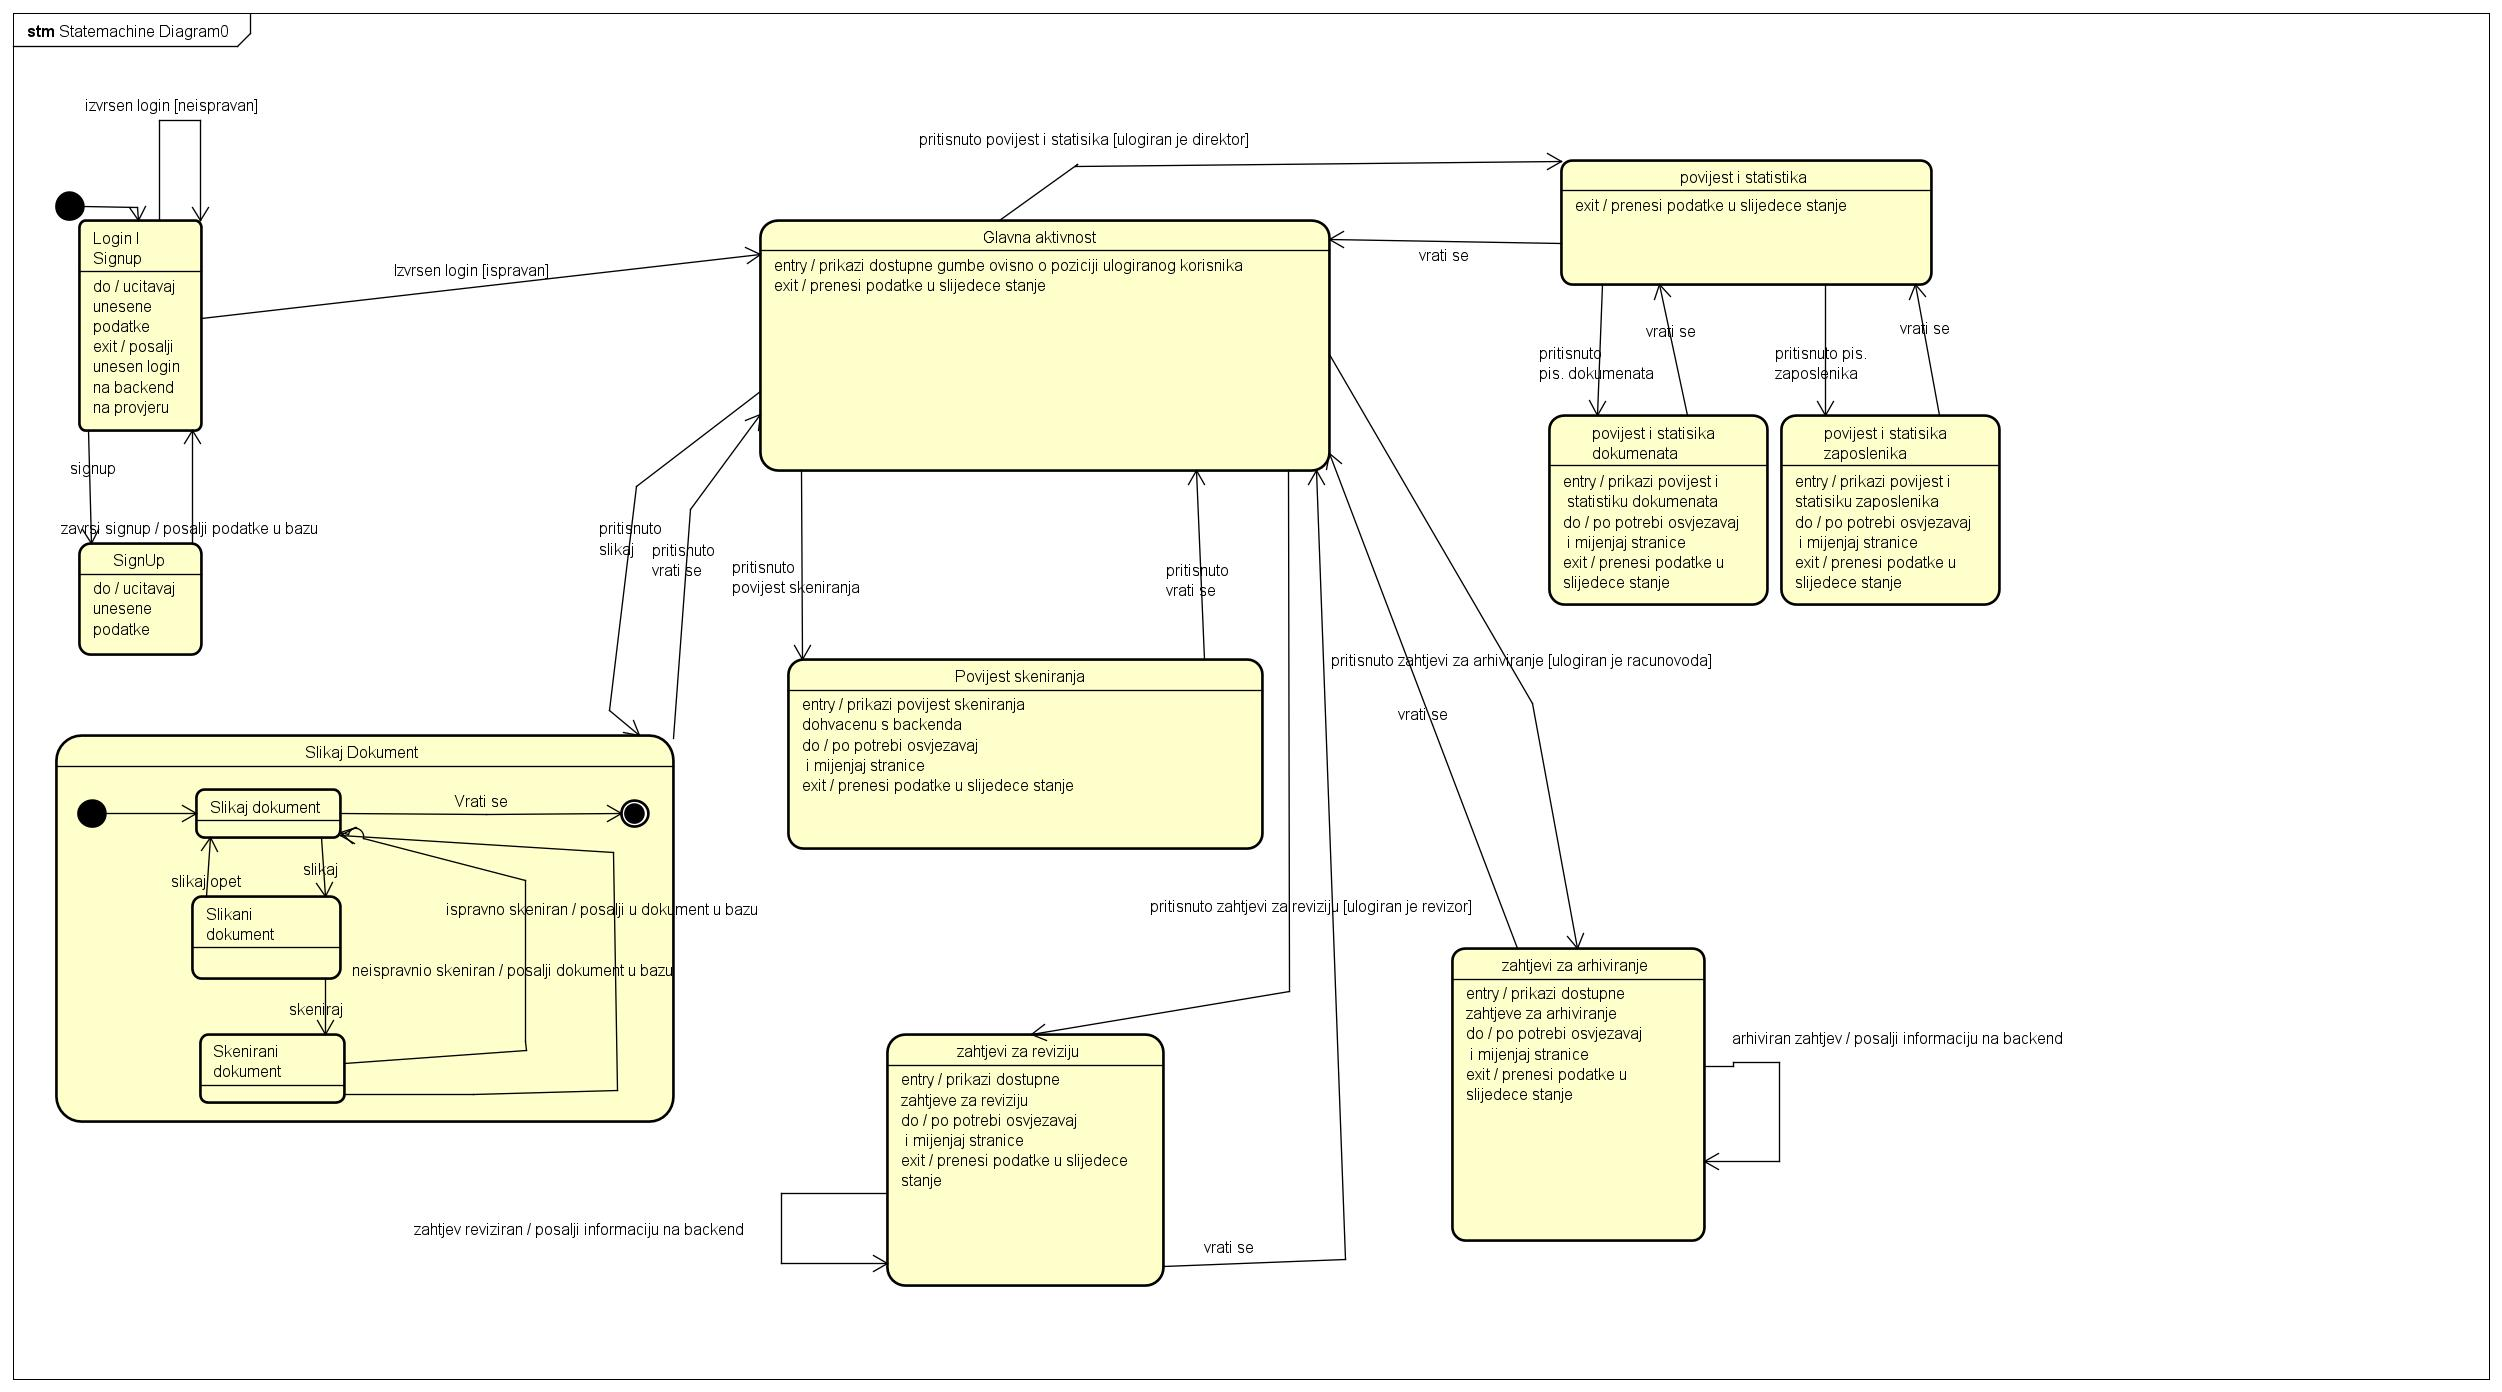
\includegraphics[width=\linewidth]{./dijagrami/Dijagram_stanja.jpg}
				\caption{Dijagram stanja}
				\label{fig:Class}
			\end{figure}
			
			\eject 
		
	\section{Dijagram aktivnosti}
	
	
	
	Dijagram aktivnosti pokazuje proces skeniranja jednog dokumenta.
		Korisnik se prvo prijavljuje u svoj korisnički račun gdje
		odabire funkciju skeniranja. Zatim korisnik slika željeni dokument i aplikacija mu prikazuje dobiveni sažetak dokumenta. 
		Korisnik završno odlučuje jeli zadovoljan sa sažetkom te se taj njegov odgovor i sažetak šalju u bazu podataka čime je završen proces skeniranja.
	
	
	\begin{figure}
		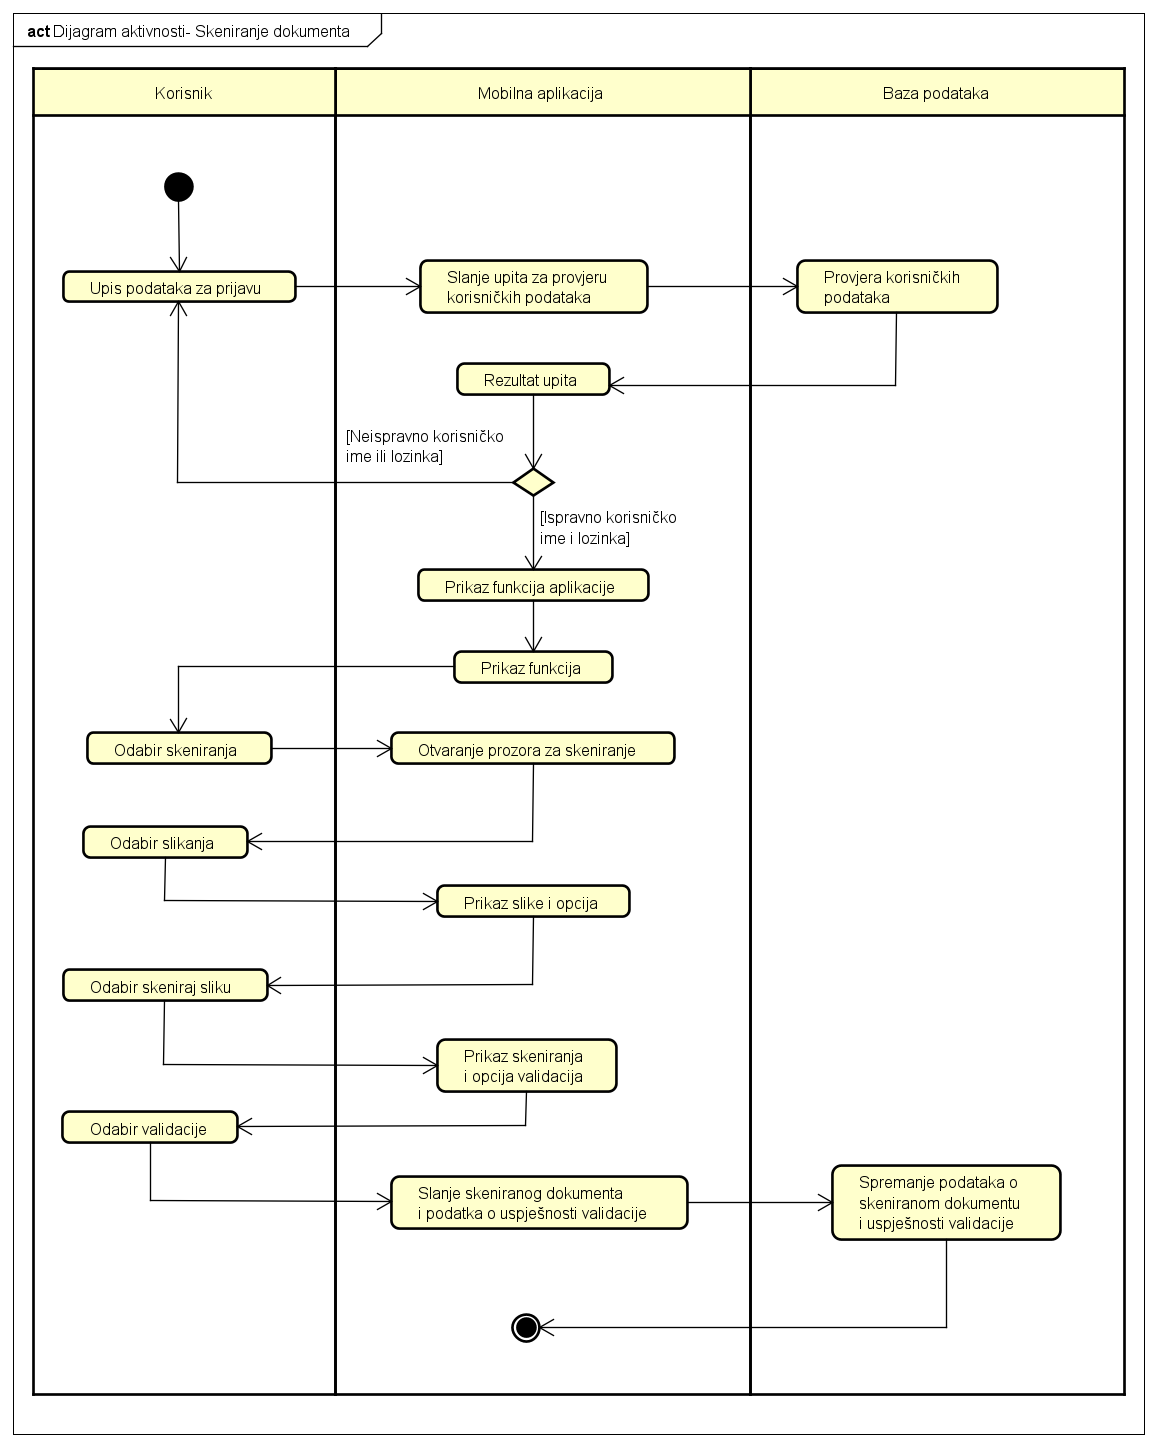
\includegraphics[width=\linewidth]{./dijagrami/dijagram_aktivnosti.png}
		\caption{Dijagram aktivnosti - Skeniranje dokumenta}
		\label{fig:Aktivnost}
	\end{figure}
	
	\eject
		\section{Dijagram komponenti}
		
			\textbf{\textit{dio 2. revizije}}\\
		
			
			 
			 Dijagram komponenti na slici 4.4 prikazuje komponente sustava te njihove međuovisnosti. Sustavu se pristupa preko komponente grafičkog sučelja koja je zadužena za prikaz sadržaja korisniku. Glavna funkcionalnost aplikacije jest mogućnost skeniranja dokumenata i njihovo spremanje u bazu podataka. Zato je grafičkom sučelju potreban API koji će mu omogućiti prepoznavanje teksta te mu je potrebno sučelje za komunikaciju s poslužiteljem, a sam nudi sučelje za slanje podataka u obliku JSON objekata. Komponenta "OCR prepoznavanje teksta" nudi sučelje za skeniranje dokumenata dok se komunikacija s poslužiteljem odvija "Dohvati JSON" i "Šalje JSON" sučelja. Komponenta "Lambda API Gateway" je zadužena za komunikaciju s bazom podataka i s grafičkim sučeljem, a za rad su joj potrebne komponente "Dokument" i "Korisnik" kako bi mogla komunicirati s bazom podataka. Baza podataka nudi sučelje preko kojeg je omogućena komunikacija s poslužiteljem.
			 
			 \begin{figure}[H]
			 	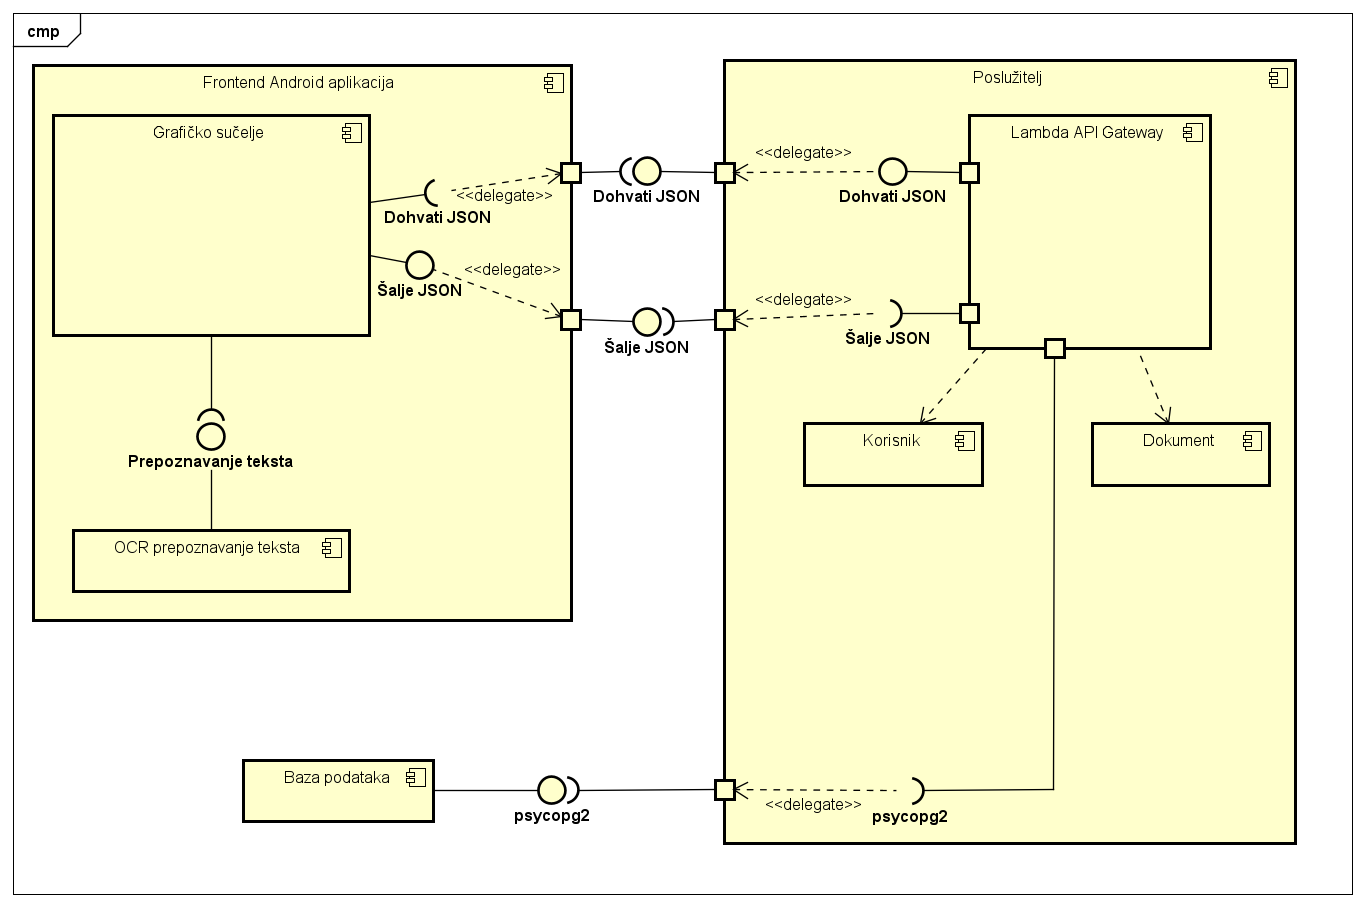
\includegraphics[width=\linewidth]{./dijagrami/Dijagram_komponenti.png}
			 	\caption{Dijagram komponenti}
			 	\label{fig:DK}
			 \end{figure}
	\chapter{Implementacija i korisničko sučelje}
		
		
		\section{Korištene tehnologije i alati}
		
			\textbf{\textit{dio 2. revizije}}
			
			Komunikacija među članovima tima realizirana je korištenjem aplikacija WhatsApp\footnote{\href{https://www.whatsapp.com/}{https://www.whatsapp.com/}} i Discord\footnote{\href{https://discord.com/}{https://discord.com/}}. Za izradu sekvencijskih dijagrama korišten je web alat za izradu dijagrama Online Visual Paradigm\footnote{\href{https://online.visual-paradigm.com/}{https://online.visual-paradigm.com/}}. Za izradu svih ostalih dijagrama korišten je program Astah\footnote{\href{https://astah.net/}{https://astah.net/}} koji služi za modeliranje i izradu dijagrama u inženjerskoj struci.
			
			Upravljanje izvornim kodom ostvareno je korištenjem sustava Git\footnote{\href{https://git-scm.com/}{https://git-scm.com/}}, a udaljeni repozitorij projekta dostupan je na web sustavu GitLab\footnote{\href{https://about.gitlab.com/}{https://about.gitlab.com/}}.\\
			
			Frontend aplikacije napravljen je u razvojnom okruženju Android Studio\footnote{\href{https://developer.android.com/studio?gclid=CjwKCAiA24SPBhB0EiwAjBgkhjQMRvsHMZCuxfC4b_03_6rtMeVgpqzEHRJTu-w7eo0ddFUCdb-aWBoC-C8QAvD_BwE&gclsrc=aw.ds}{Android Studio}} koristeći programski jezik Java\footnote{\href{https://www.java.com/en/}{https://www.java.com/en/}}. Android Studio je službeno razvojno okruženje za Android platformu i temelji se na InteliJ IDEA-u. Prvenstveno se koristi za izradu Android aplikacija i igara. Pri razvoju softvera Android Studio koristi Gradle tehnologiju, predloške koda s GitHub-a i podršku za korištenje Google Cloud platforme.\\ 
			
			Backend aplikacije je napisan programskim jezikom Python\footnote{\href{https://www.python.org/}{https://www.python.org/}} u razvojnom okruženju Visual Studio Code\footnote{\href{https://code.visualstudio.com/}{https://code.visualstudio.com/}}. Visual Studio Code se najviše koristi za pisanje i debbugiranje programskog koda aplikacija. Uz standardne funkcionalnosti Pythona korišten je i adapter za komunikaciju s bazom podataka Psycopg2\footnote{\href{https://pypi.org/project/psycopg2/}{https://pypi.org/project/psycopg2/}}.\\
			
			Dodatno je za ostvarenje backenda korištena i cloud platforma Amazon AWS\footnote{\href{https://aws.amazon.com}{Amazon AWS}}. Konkretno su korištene usluge AWS Lambda\footnote{\href{https://aws.amazon.com/lambda/?nc2=h\_ql\_prod\_fs\_lbd}{https://aws.amazon.com/lambda/?nc2=h\_ql\_prod\_fs\_lbd}}, API Gateway\footnote{\href{https://aws.amazon.com/api-gateway/?nc2=type\_a}{https://aws.amazon.com/api-gateway/?nc2=type\_a}} i RDS Database\footnote{\href{https://aws.amazon.com/rds/?nc2=type\_a}{https://aws.amazon.com/rds/?nc2=type\_a}}. API Gateway služi za preusmjeravanje HTTP zahtjeva s frontenda na AWS Lambdu u kojoj su implementirane funkcionalnosti backenda. AWS Lambda zatim preko istog API Gatewaya šalje odgovor frontendu. \\
			
			Baza podataka nalazi se na poslužitelju Amazon RDS.
			
			\eject 
		
	
		\section{Ispitivanje programskog rješenja}
			
			\textbf{\textit{dio 2. revizije}}\\
			
			
	
			
			\subsection{Ispitivanje komponenti}
			
			\textbf{Ispitni slučaj 1: Registracija novog korisnika}\\
			\begin{itemize}
				\item funkciji register\_handler predaju se podaci o korsiniku u JSON formatu
				\item funkcija stvara element klase User i poziva metodu register
			
			\item očekivani rezultat:\\
				\begin{itemize}
					\item funkcija vraća poruku "SignupValid" 
					\item korisnik se upisuje u bazu podataka
				\end{itemize}
			\item rezultat:
		\end{itemize}
			\begin{figure}[H]
				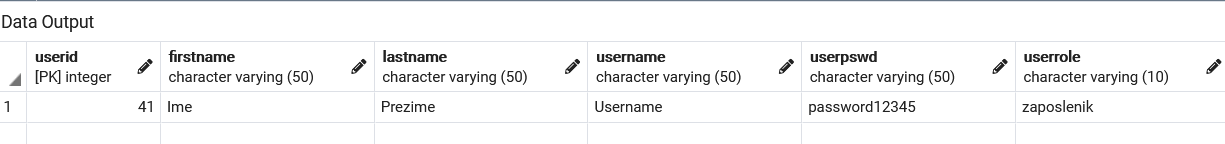
\includegraphics[scale=0.5]{./slike/baza1.png}
				\caption{Rezultat u bazi podataka}
				\label{fig:REZ1}
			\end{figure}

			\begin{figure}[H]
				\centering
				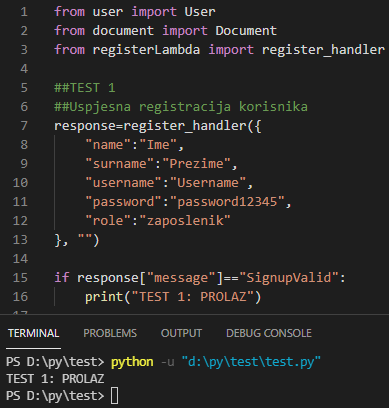
\includegraphics[scale=0.5]{./slike/rez1.png}
				\caption{Rezultat u razvojnom okruženju}
				\label{fig:REZ1}
			\end{figure}
		
		
		\textbf{Ispitni slučaj 2: Pokušaj registracije s već postojećim korisničkim imenom:}\\
		\begin{itemize}
			\item funkciji register\_handler predaju se podaci o korsiniku u JSON formatu
			\item funkcija stvara element klase User i poziva metodu register
			
			\item očekivani rezultat:\\
			\begin{itemize}
				\item funkcija vraća poruku "SignupInvalid" 
				\item korisnik se ne upisuje u bazu podataka
			\end{itemize}
			\item rezultat:
		\end{itemize}
		\begin{figure}[H]
			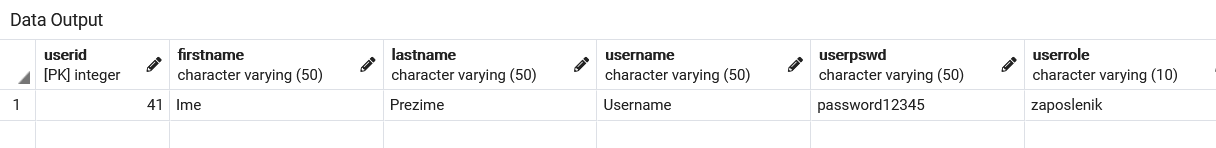
\includegraphics[scale=0.5]{./slike/baza2.png}
			\caption{Potvrda rezultata u bazi podataka}
			\label{fig:REZ2}
		\end{figure}
		
		\begin{figure}[H]
			\centering
			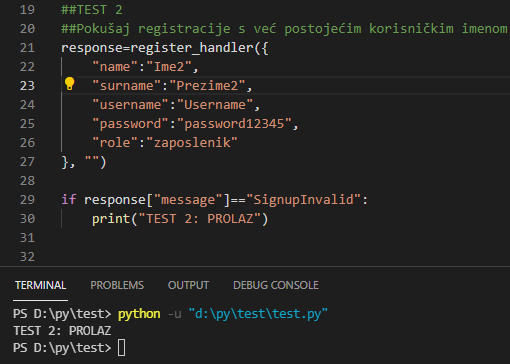
\includegraphics[scale=0.5]{./slike/rez2.png}
			\caption{Rezultat u razvojnom okruženju}
			\label{fig:REZ2}
		\end{figure}
	
	
		\textbf{Ispitni slučaj 3: Login postojećeg korisnika:}\\
\begin{itemize}
	\item funkciji login\_handler predaju se podaci o korsiniku u JSON formatu
	\item funkcija dohvaća korisnika iz baze koristeći korisničko ime
	
	\item očekivani rezultat:\\
	\begin{itemize}
		\item funkcija vraća poruku "LoginValid" 
		\item uz poruku vraća i podatke o korisniku
	\end{itemize}
	\item rezultat:
\end{itemize}
\begin{figure}[H]
	\centering
	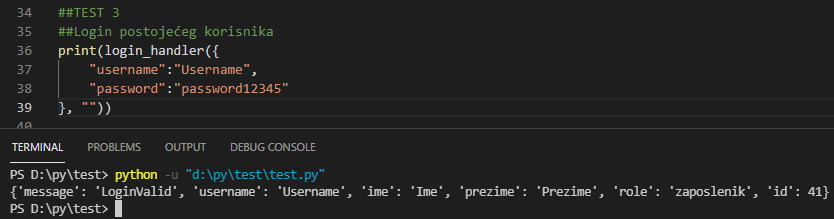
\includegraphics[scale=0.5]{./slike/rez3.png}
	\caption{Rezultat u razvojnom okruženju}
	\label{fig:REZ3}
\end{figure}


		\textbf{Ispitni slučaj 4: Login nepostojećeg korisnika:}\\
\begin{itemize}
	\item funkciji login\_handler predaju se podaci o korsiniku u JSON formatu
	\item funkcija pokušava dohvatiti korisnika iz baze koristeći korisničko ime
	
	\item očekivani rezultat:\\
	\begin{itemize}
		\item funkcija vraća poruku "LoginInvalid" 
		\item uz poruku vraća i prazne podatke o korisniku
	\end{itemize}
	\item rezultat:
\end{itemize}
\begin{figure}[H]
	\centering
	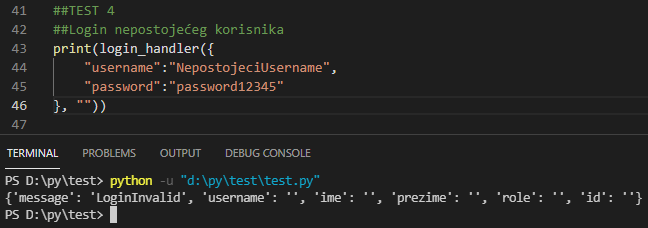
\includegraphics[scale=0.5]{./slike/rez4.png}
	\caption{Rezultat u razvojnom okruženju}
	\label{fig:REZ4}
\end{figure}


		\textbf{Ispitni slučaj 5: Pokušaj logina postojećeg korisnika s neispravnom lozinkom:}\\
\begin{itemize}
	\item funkciji login\_handler predaju se podaci o korsiniku u JSON formatu
	\item funkcija dohvaća korisnika iz baze podataka koristeći korisničko ime i uspoređuje lozinke 
	
	\item očekivani rezultat:\\
	\begin{itemize}
		\item funkcija vraća poruku "LoginInvalid" 
		\item uz poruku vraća i podatke o korisniku jer korisnik postoji, samo je lozinka neispravna
	\end{itemize}
	\item rezultat:
\end{itemize}
\begin{figure}[H]
	\centering
	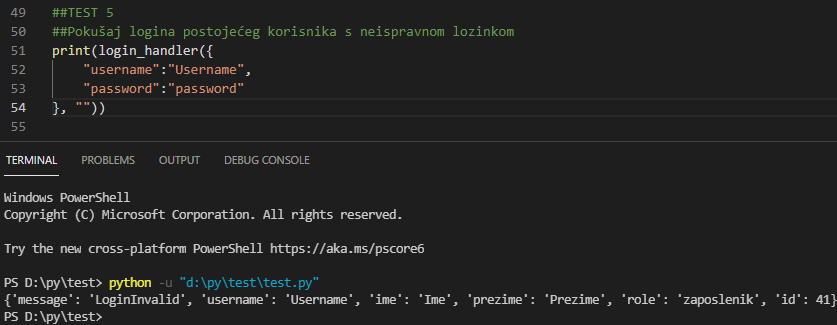
\includegraphics[scale=0.5]{./slike/rez5.png}
	\caption{Rezultat u razvojnom okruženju}
	\label{fig:REZ5}
\end{figure}


		\textbf{Ispitni slučaj 6: Dodavanje ispravno skeniranog dokumenta:}\\
\begin{itemize}
	\item funkciji add\_document\_handler predaju se podaci o dokumentu, datum skeniranja i ID korisnika koji je skenirao dokument
	\item funkcija stvara objekt klase Document i poziva metodu addDocument
	\item funkcija addDocument dodaje zapis o skeniranju u relacije "scanhistory", "documents" i, ako je dokument označen kao ispravan, u relaciju "reviserpending" ili "accountantpending" 
	
	\item očekivani rezultat:\\
	\begin{itemize}
		\item funkcija dodaje zapise o skeniranju dokumenta u relacije "scanhistory", "documents" i, pošto je korisnik koji je skenirao dokument zaposlenik, u relaciju "reviserpending"
	\end{itemize}
	\item rezultat:
\end{itemize}
\begin{figure}[H]
	\centering
	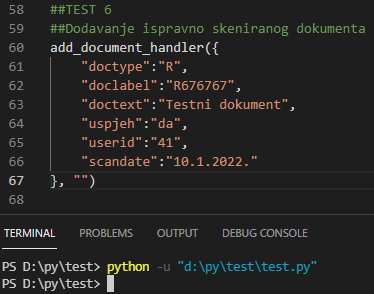
\includegraphics[scale=0.5]{./slike/rez6.png}
	\caption{Rezultat u razvojnom okruženju}
	\label{fig:REZ6}
\end{figure}
\begin{figure}[H]
	\centering
	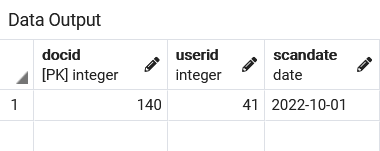
\includegraphics[scale=0.5]{./slike/baza6sh.png}
	\caption{Rezultat u relaciji "scanhistory"}
	\label{fig:BAZA6a}
\end{figure}
\begin{figure}[H]
	\centering
	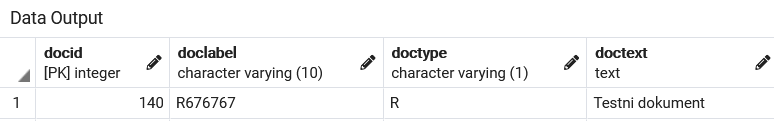
\includegraphics[scale=0.5]{./slike/baza6doc.png}
	\caption{Rezultat u relaciji "documents"}
	\label{fig:BAZA6b}
\end{figure}
\begin{figure}[H]
	\centering
	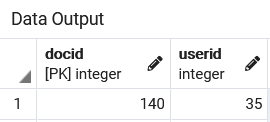
\includegraphics[scale=0.5]{./slike/baza6rp.png}
	\caption{Rezultat u relaciji "reviserpending"}
	\label{fig:BAZA6c}
\end{figure}


		\textbf{Ispitni slučaj 7: Dodavanje neispravno skeniranog dokumenta:}\\
\begin{itemize}
	\item funkciji add\_document\_handler predaju se podaci o dokumentu, datum skeniranja i ID korisnika koji je skenirao dokument
	\item funkcija stvara objekt klase Document i poziva metodu addDocument
	\item funkcija addDocument dodaje zapis o skeniranju u relacije "scanhistory", "documents" i, ako je dokument označen kao ispravan, u relaciju "reviserpending" ili "accountantpending" 
	
	\item očekivani rezultat:\\
	\begin{itemize}
		\item funkcija dodaje zapise o skeniranju dokumenta u relacije "scanhistory", "documents" i, pošto je dokument označen kao pogrešno skeniran, ne dodaje ga u relaciju "reviserpending"
	\end{itemize}
	\item rezultat:
	\begin{itemize}
		\item funkcija je prošla test
	\end{itemize}
\end{itemize}
\begin{figure}[H]
	\centering
	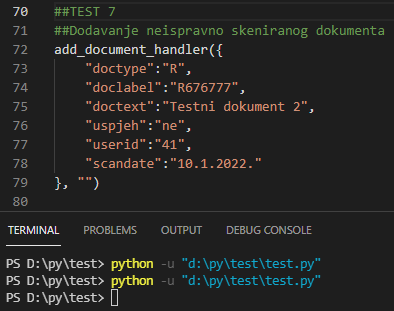
\includegraphics[scale=0.5]{./slike/rez7.png}
	\caption{Rezultat u razvojnom okruženju}
	\label{fig:REZ7}
\end{figure}
\begin{figure}[H]
	\centering
	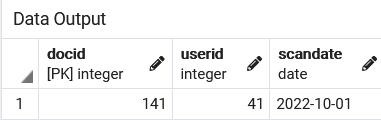
\includegraphics[scale=0.5]{./slike/baza7sh.png}
	\caption{Rezultat u relaciji "scanhistory"}
	\label{fig:BAZA7a}
\end{figure}
\begin{figure}[H]
	\centering
	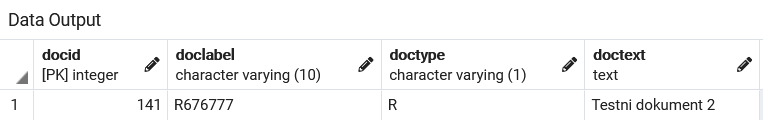
\includegraphics[scale=0.5]{./slike/baza7doc.png}
	\caption{Rezultat u relaciji "documents"}
	\label{fig:BAZA7b}
\end{figure}
\begin{figure}[H]
	\centering
	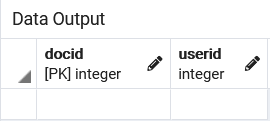
\includegraphics[scale=0.5]{./slike/baza7rp.png}
	\caption{Rezultat u relaciji "reviserpending"}
	\label{fig:BAZA7c}
\end{figure}


	\textbf{Ispitni slučaj 8: Slučajno dodavanje dokumenta kao ispravnog iako je oznaka dokumenta pogrešno skenirana:}\\
\begin{itemize}
	\item funkciji add\_document\_handler predaju se podaci o dokumentu, datum skeniranja i ID korisnika koji je skenirao dokument
	\item funkcija stvara objekt klase Document i poziva metodu addDocument
	\item funkcija addDocument dodaje zapis o skeniranju u relacije "scanhistory", "documents" i, ako je dokument označen kao ispravan, u relaciju "reviserpending" ili "accountantpending"
	\item pošto je oznaka dokumenta pogrešno skenirana, frontend aplikacije backendu šalje prazan string kao atribut "doclabel"
	
	\item očekivani rezultat:\\
	\begin{itemize}
		\item funkcija dodaje zapise o skeniranju dokumenta u relacije "scanhistory", "documents" i, unatoč tome što je dokument označen kao ispravno skeniran, ne dodaje ga u relaciju "reviserpending" jer je "doclabel" prazan string
		\item vrijednosti "doclabel" i "doctype" su u relaciji document postavljene kao null vrijednosti
	\end{itemize}
	\item rezultat:
	\begin{itemize}
		\item funkcija je prošla test
	\end{itemize}
\end{itemize}
\begin{figure}[H]
	\centering
	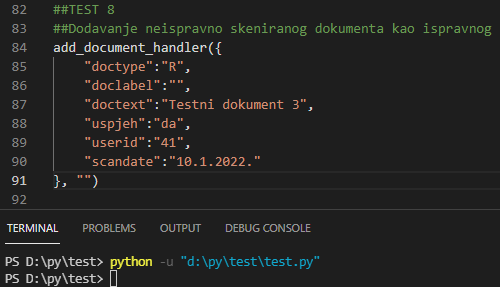
\includegraphics[scale=0.5]{./slike/rez8.png}
	\caption{Rezultat u razvojnom okruženju}
	\label{fig:REZ8}
\end{figure}
\begin{figure}[H]
	\centering
	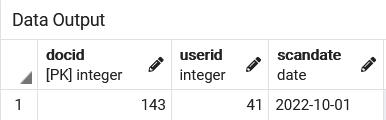
\includegraphics[scale=0.5]{./slike/baza8sh.png}
	\caption{Rezultat u relaciji "scanhistory"}
	\label{fig:BAZA8a}
\end{figure}
\begin{figure}[H]
	\centering
	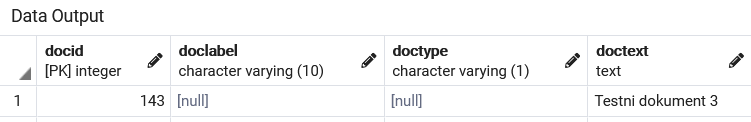
\includegraphics[scale=0.5]{./slike/baza8doc.png}
	\caption{Rezultat u relaciji "documents"}
	\label{fig:BAZA8b}
\end{figure}
\begin{figure}[H]
	\centering
	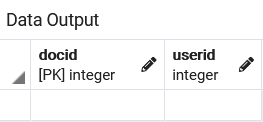
\includegraphics[scale=0.5]{./slike/baza8rp.png}
	\caption{Rezultat u relaciji "reviserpending"}
	\label{fig:BAZA8c}
\end{figure}
			
		
			
			\subsection{Ispitivanje sustava}
			\subsubsection{Testiranje logina}
			Testiramo može li se korisnik prijaviti u aplikaciju.
			\begin{lstlisting}[language=Java]
				@LargeTest
				@RunWith(AndroidJUnit4.class)
				public class login_radnik_test {
					
					@Rule
					public ActivityTestRule<MainActivity> mActivityTestRule = new ActivityTestRule<>(MainActivity.class);
					
					@Test
					public void login_radnik_test() {
						ViewInteraction appCompatEditText = onView(
						allOf(withId(R.id.etUsername),
						childAtPosition(
						allOf(withId(R.id.LogInText),
						childAtPosition(
						withId(android.R.id.content),
						0)),
						1),
						isDisplayed()));
						appCompatEditText.perform(replaceText("radnik"), closeSoftKeyboard());
						
						ViewInteraction appCompatEditText2 = onView(
						allOf(withId(R.id.etPassword),
						childAtPosition(
						allOf(withId(R.id.LogInText),
						childAtPosition(
						withId(android.R.id.content),
						0)),
						2),
						isDisplayed()));
						appCompatEditText2.perform(replaceText("rad1234"), closeSoftKeyboard());
						
						ViewInteraction appCompatEditText3 = onView(
						allOf(withId(R.id.etPassword), withText("rad1234"),
						childAtPosition(
						allOf(withId(R.id.LogInText),
						childAtPosition(
						withId(android.R.id.content),
						0)),
						2),
						isDisplayed()));
						appCompatEditText3.perform(pressImeActionButton());
						
						ViewInteraction materialButton = onView(
						allOf(withId(R.id.LoginBtn), withText("Log In"),
						childAtPosition(
						allOf(withId(R.id.LogInText),
						childAtPosition(
						withId(android.R.id.content),
						0)),
						3),
						isDisplayed()));
						materialButton.perform(click());
					}
					
					private static Matcher<View> childAtPosition(
					final Matcher<View> parentMatcher, final int position) {
						
						return new TypeSafeMatcher<View>() {
							@Override
							public void describeTo(Description description) {
								description.appendText("Child at position " + position + " in parent ");
								parentMatcher.describeTo(description);
							}
							
							@Override
							public boolean matchesSafely(View view) {
								ViewParent parent = view.getParent();
								return parent instanceof ViewGroup && parentMatcher.matches(parent)
								&& view.equals(((ViewGroup) parent).getChildAt(position));
							}
						};
					}
				}
			\end{lstlisting}
		
		Ako je login ispravan, proći ćemo test.
		
		\begin{figure}[H]
			\centering
			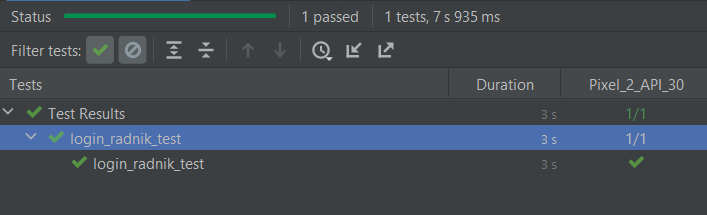
\includegraphics[scale=0.5]{./slike/test1.png}
			\caption{"Test logina"}
			\label{fig:test1}
		\end{figure}\eject
	
		\subsubsection{Testiranje prisutnosti slike u ImageView-u}
	Testiramo je li slika prisutna u ImageView-u.
	\begin{lstlisting}[language=Java]
	@LargeTest
	@RunWith(AndroidJUnit4.class)
	public class prikazuje_sliku_test {
		
		@Rule
		public ActivityTestRule<MainActivity> mActivityTestRule = new ActivityTestRule<>(MainActivity.class);
		
		@Rule
		public GrantPermissionRule mGrantPermissionRule =
		GrantPermissionRule.grant(
		"android.permission.CAMERA");
		
		@Test
		public void prikazuje_sliku_test() {
			ViewInteraction appCompatEditText = onView(
			allOf(withId(R.id.etUsername),
			childAtPosition(
			allOf(withId(R.id.LogInText),
			childAtPosition(
			withId(android.R.id.content),
			0)),
			1),
			isDisplayed()));
			appCompatEditText.perform(replaceText("radnik"), closeSoftKeyboard());
			
			ViewInteraction appCompatEditText2 = onView(
			allOf(withId(R.id.etPassword),
			childAtPosition(
			allOf(withId(R.id.LogInText),
			childAtPosition(
			withId(android.R.id.content),
			0)),
			2),
			isDisplayed()));
			appCompatEditText2.perform(replaceText("rad1234"), closeSoftKeyboard());
			
			ViewInteraction materialButton = onView(
			allOf(withId(R.id.LoginBtn), withText("Log In"),
			childAtPosition(
			allOf(withId(R.id.LogInText),
			childAtPosition(
			withId(android.R.id.content),
			0)),
			3),
			isDisplayed()));
			materialButton.perform(click());
			
			ViewInteraction materialButton2 = onView(
			allOf(withId(R.id.ScanZap), withText("Skeniranje"),
			childAtPosition(
			childAtPosition(
			withId(android.R.id.content),
			0),
			0),
			isDisplayed()));
			materialButton2.perform(click());
			
			try {
				TimeUnit.SECONDS.sleep(2);
			} catch (InterruptedException e) {
				e.printStackTrace();
			}
			
			ViewInteraction materialButton3 = onView(withId(R.id.SlikajButton));
			materialButton3.perform(click());
			try {
				TimeUnit.SECONDS.sleep(2);
			} catch (InterruptedException e) {
				e.printStackTrace();
			}
			onView(withId(R.id.SlikaWind)).check(matches(notNullValue()));
		}
		
		private static Matcher<View> childAtPosition(
		final Matcher<View> parentMatcher, final int position) {
			
			return new TypeSafeMatcher<View>() {
				@Override
				public void describeTo(Description description) {
					description.appendText("Child at position " + position + " in parent ");
					parentMatcher.describeTo(description);
				}
				
				@Override
				public boolean matchesSafely(View view) {
					ViewParent parent = view.getParent();
					return parent instanceof ViewGroup && parentMatcher.matches(parent)
					&& view.equals(((ViewGroup) parent).getChildAt(position));
				}
			};
		}
	}
	\end{lstlisting}
	
	Ako je slika u ImageView-u, proći ćemo test.
	
	\begin{figure}[H]
		\centering
		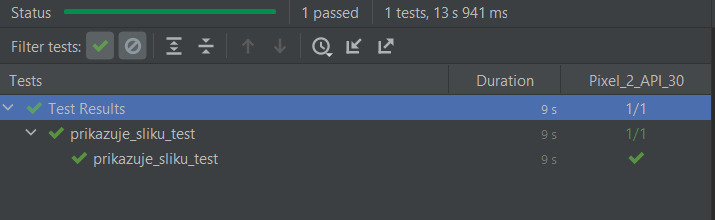
\includegraphics[scale=0.5]{./slike/test2.png}
		\caption{"Test prisutnosti slike u ImageView-u"}
		\label{fig:test2}
	\end{figure}\eject


	\subsubsection{Testiranje ispravnog skena dokumenta}
Testiramo je li skenirani dokument ispravan.
Ispravan dokument je:\\
Internal file in our app\\
INT9852
\begin{lstlisting}[language=Java]
@LargeTest
@RunWith(AndroidJUnit4.class)
public class ispravanSkenTest {
	
	@Rule
	public ActivityTestRule<MainActivity> mActivityTestRule = new ActivityTestRule<>(MainActivity.class);
	
	@Rule
	public GrantPermissionRule mGrantPermissionRule =
	GrantPermissionRule.grant(
	"android.permission.CAMERA");
	
	@Test
	public void ispravanSkenTest() {
		ViewInteraction appCompatEditText = onView(
		allOf(withId(R.id.etUsername),
		childAtPosition(
		allOf(withId(R.id.LogInText),
		childAtPosition(
		withId(android.R.id.content),
		0)),
		1),
		isDisplayed()));
		appCompatEditText.perform(replaceText("user12"), closeSoftKeyboard());
		
		ViewInteraction appCompatEditText2 = onView(
		allOf(withId(R.id.etPassword),
		childAtPosition(
		allOf(withId(R.id.LogInText),
		childAtPosition(
		withId(android.R.id.content),
		0)),
		2),
		isDisplayed()));
		appCompatEditText2.perform(replaceText("user12"), closeSoftKeyboard());
		
		ViewInteraction materialButton = onView(
		allOf(withId(R.id.LoginBtn), withText("Log In"),
		childAtPosition(
		allOf(withId(R.id.LogInText),
		childAtPosition(
		withId(android.R.id.content),
		0)),
		3),
		isDisplayed()));
		materialButton.perform(click());
		
		ViewInteraction materialButton2 = onView(
		allOf(withId(R.id.ScanZap), withText("Skeniranje"),
		childAtPosition(
		childAtPosition(
		withId(android.R.id.content),
		0),
		0),
		isDisplayed()));
		materialButton2.perform(click());
		try {
			TimeUnit.SECONDS.sleep(10);
		} catch (InterruptedException e) {
			e.printStackTrace();
		}
		ViewInteraction materialButton3 = onView(
		allOf(withId(R.id.SlikajButton), withText("SLIKAJ"),
		childAtPosition(
		childAtPosition(
		withId(android.R.id.content),
		0),
		1),
		isDisplayed()));
		materialButton3.perform(click());
		try {
			TimeUnit.SECONDS.sleep(3);
		} catch (InterruptedException e) {
			e.printStackTrace();
		}
		
		ViewInteraction materialButton4 = onView(
		allOf(withId(R.id.SkenirajSlikuButton), withText("Skeniraj Sliku"),
		childAtPosition(
		childAtPosition(
		withId(android.R.id.content),
		0),
		2),
		isDisplayed()));
		materialButton4.perform(click());
		try {
			TimeUnit.SECONDS.sleep(3);
		} catch (InterruptedException e) {
			e.printStackTrace();
		}
		ViewInteraction textView = onView(
		allOf(withId(R.id.SkeniraniTekst),
		withParent(withParent(withId(android.R.id.content))),
		isDisplayed()));
		textView.check(matches(withText("Internal file in our app\nINT9852\n")));
		try {
			TimeUnit.SECONDS.sleep(3);
		} catch (InterruptedException e) {
			e.printStackTrace();
		}
		ViewInteraction materialButton5 = onView(
		allOf(withId(R.id.IspravanScanButton), withText("Ispravan Scan"),
		childAtPosition(
		childAtPosition(
		withId(android.R.id.content),
		0),
		1),
		isDisplayed()));
		materialButton5.perform(click());
		try {
			TimeUnit.SECONDS.sleep(3);
		} catch (InterruptedException e) {
			e.printStackTrace();
		}
	}
	
	private static Matcher<View> childAtPosition(
	final Matcher<View> parentMatcher, final int position) {
		
		return new TypeSafeMatcher<View>() {
			@Override
			public void describeTo(Description description) {
				description.appendText("Child at position " + position + " in parent ");
				parentMatcher.describeTo(description);
			}
			
			@Override
			public boolean matchesSafely(View view) {
				ViewParent parent = view.getParent();
				return parent instanceof ViewGroup && parentMatcher.matches(parent)
				&& view.equals(((ViewGroup) parent).getChildAt(position));
			}
		};
	}
}

\end{lstlisting}

Ako je skenirani dokument ispravan, proći ćemo test.

\begin{figure}[H]
	\centering
	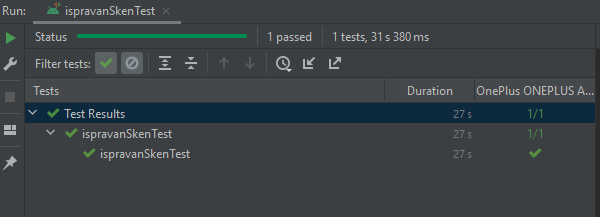
\includegraphics[scale=1]{./slike/test3.png}
	\caption{"Test ispravnosti skeniranog dokumenta"}
	\label{fig:test3}
\end{figure}\eject


	\subsubsection{Testiranje neispravnog skena dokumenta}
Testiramo je li skenirani dokument neispravan.
Ispravan dokument je:\\
Internal file in our app\\
INT9852
\begin{lstlisting}[language=Java]
	@LargeTest
	@RunWith(AndroidJUnit4.class)
	public class neispravanSkenTest {
		
		@Rule
		public ActivityTestRule<MainActivity> mActivityTestRule = new ActivityTestRule<>(MainActivity.class);
		
		@Rule
		public GrantPermissionRule mGrantPermissionRule =
		GrantPermissionRule.grant(
		"android.permission.CAMERA");
		
		@Test
		public void neispravanSkenTest() {
			ViewInteraction appCompatEditText = onView(
			allOf(withId(R.id.etUsername),
			childAtPosition(
			allOf(withId(R.id.LogInText),
			childAtPosition(
			withId(android.R.id.content),
			0)),
			1),
			isDisplayed()));
			appCompatEditText.perform(replaceText("user12"), closeSoftKeyboard());
			
			ViewInteraction appCompatEditText2 = onView(
			allOf(withId(R.id.etPassword),
			childAtPosition(
			allOf(withId(R.id.LogInText),
			childAtPosition(
			withId(android.R.id.content),
			0)),
			2),
			isDisplayed()));
			appCompatEditText2.perform(replaceText("user12"), closeSoftKeyboard());
			
			ViewInteraction appCompatEditText3 = onView(
			allOf(withId(R.id.etPassword), withText("user12"),
			childAtPosition(
			allOf(withId(R.id.LogInText),
			childAtPosition(
			withId(android.R.id.content),
			0)),
			2),
			isDisplayed()));
			appCompatEditText3.perform(pressImeActionButton());
			
			ViewInteraction materialButton = onView(
			allOf(withId(R.id.LoginBtn), withText("Log In"),
			childAtPosition(
			allOf(withId(R.id.LogInText),
			childAtPosition(
			withId(android.R.id.content),
			0)),
			3),
			isDisplayed()));
			materialButton.perform(click());
			
			ViewInteraction materialButton2 = onView(
			allOf(withId(R.id.ScanZap), withText("Skeniranje"),
			childAtPosition(
			childAtPosition(
			withId(android.R.id.content),
			0),
			0),
			isDisplayed()));
			materialButton2.perform(click());
			try {
				TimeUnit.SECONDS.sleep(10);
			} catch (InterruptedException e) {
				e.printStackTrace();
			}
			ViewInteraction materialButton3 = onView(
			allOf(withId(R.id.SlikajButton), withText("SLIKAJ"),
			childAtPosition(
			childAtPosition(
			withId(android.R.id.content),
			0),
			1),
			isDisplayed()));
			materialButton3.perform(click());
			try {
				TimeUnit.SECONDS.sleep(3);
			} catch (InterruptedException e) {
				e.printStackTrace();
			}
			
			ViewInteraction materialButton4 = onView(
			allOf(withId(R.id.SkenirajSlikuButton), withText("Skeniraj Sliku"),
			childAtPosition(
			childAtPosition(
			withId(android.R.id.content),
			0),
			2),
			isDisplayed()));
			materialButton4.perform(click());
			try {
				TimeUnit.SECONDS.sleep(3);
			} catch (InterruptedException e) {
				e.printStackTrace();
			}
			
			ViewInteraction textView = onView(
			allOf(withId(R.id.SkeniraniTekst),
			withParent(withParent(withId(android.R.id.content))),
			isDisplayed()));
			textView.check(matches(not(withText("Internal file in our app\nINT9852\n"))));
			try {
				TimeUnit.SECONDS.sleep(3);
			} catch (InterruptedException e) {
				e.printStackTrace();
			}
			
			ViewInteraction materialButton5 = onView(
			allOf(withId(R.id.NeispravanScanButton), withText("NeIspravan Scan"),
			childAtPosition(
			childAtPosition(
			withId(android.R.id.content),
			0),
			0),
			isDisplayed()));
			materialButton5.perform(click());
			try {
				TimeUnit.SECONDS.sleep(3);
			} catch (InterruptedException e) {
				e.printStackTrace();
			}
		}
		
		private static Matcher<View> childAtPosition(
		final Matcher<View> parentMatcher, final int position) {
			
			return new TypeSafeMatcher<View>() {
				@Override
				public void describeTo(Description description) {
					description.appendText("Child at position " + position + " in parent ");
					parentMatcher.describeTo(description);
				}
				
				@Override
				public boolean matchesSafely(View view) {
					ViewParent parent = view.getParent();
					return parent instanceof ViewGroup && parentMatcher.matches(parent)
					&& view.equals(((ViewGroup) parent).getChildAt(position));
				}
			};
		}
	}
	
\end{lstlisting}

Ako je skenirani dokument neispravan, npr. neki račun, proći ćemo test.

\begin{figure}[H]
	\centering
	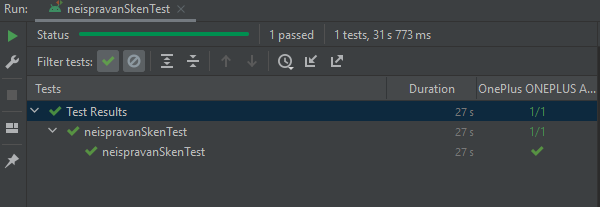
\includegraphics[scale=1]{./slike/test4.png}
	\caption{"Test neispravnosti skeniranog dokumenta"}
	\label{fig:test4}
\end{figure}\eject

Ako bi kojim slučajem skenirali traženi dokument, rezultat ne bi prošao test.

\begin{figure}[H]
	\centering
	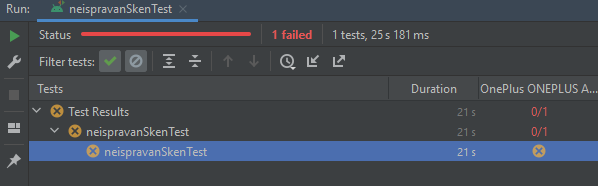
\includegraphics[scale=1]{./slike/test5.png}
	\caption{"Test neispravnosti skeniranog dokumenta"}
	\label{fig:test5}
\end{figure}\eject





	
		
		
		
		
		
		
			
			
			\eject 
		
		
	\section{Dijagram razmještaja}
	
	
	Klijent preko svojeg uređaja pristupa aplikaciji. Aplikacija se spaja na API Gateway koji je u sklopu Awsovog clouda. Unutar clouda se nalazi još virtualna mašina koja pokreće odgovarajuće lambda funkcije koje manipuliraju s bazom podataka koja je također dio clouda.
	
	\eject
	
	
	\begin{figure}
		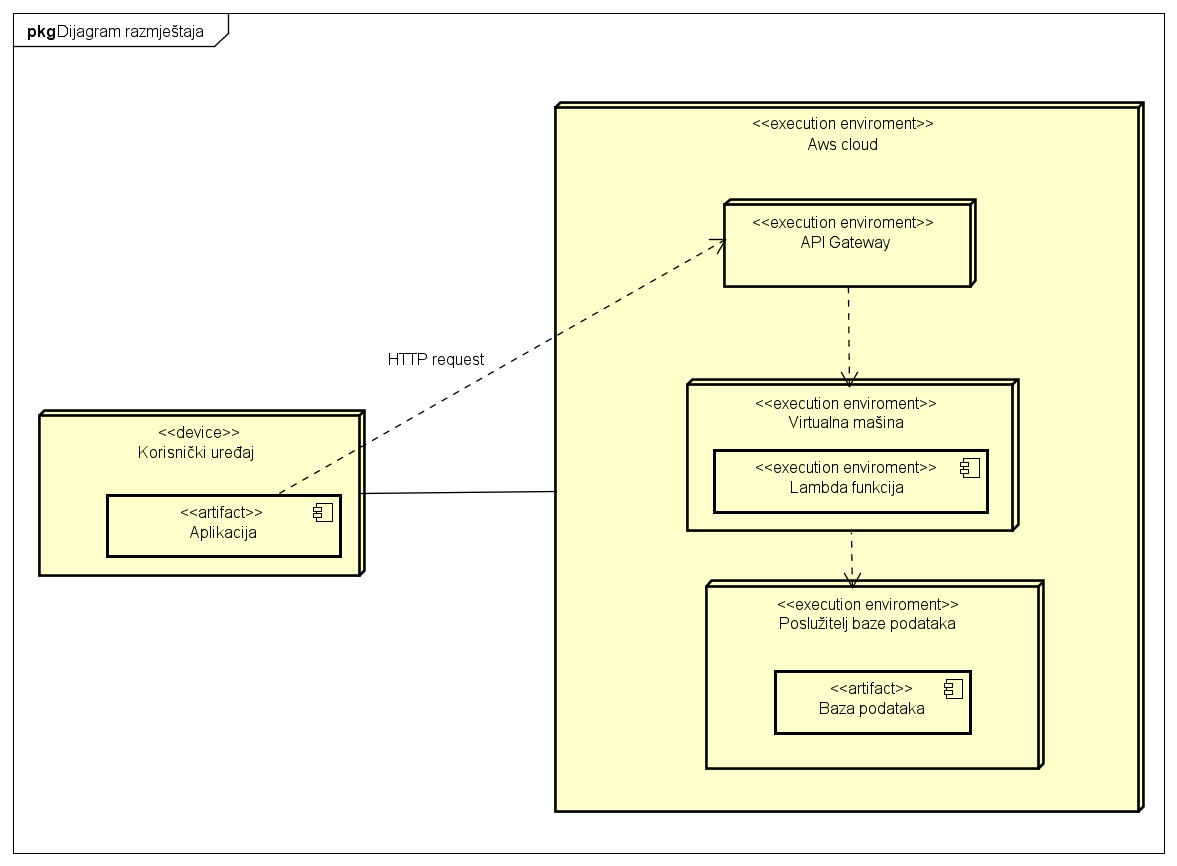
\includegraphics[width=\linewidth]{./dijagrami/dijagram_razmjestaja.png}
		\caption{Dijagram razmještaja}
		\label{fig:Raz}
	\end{figure}
	
	\eject
		
		\section{Upute za puštanje u pogon}
		
			\textbf{\textit{dio 2. revizije}}\\
		
		
			 
			 \subsection{Izgradnja aplikacije} 
			 
			 Kako bi se aplikacija izgradila, mora se prvo otvoriti u programu Android Studio, njezina putanja je :
			 \begin{itemize}
			 	\item  \path{is2-digitalizacija\IzvorniKod\Frontend\UI\SeptabilApp}.
			 \end{itemize}
			 
			\begin{figure}[H]
				\centering
				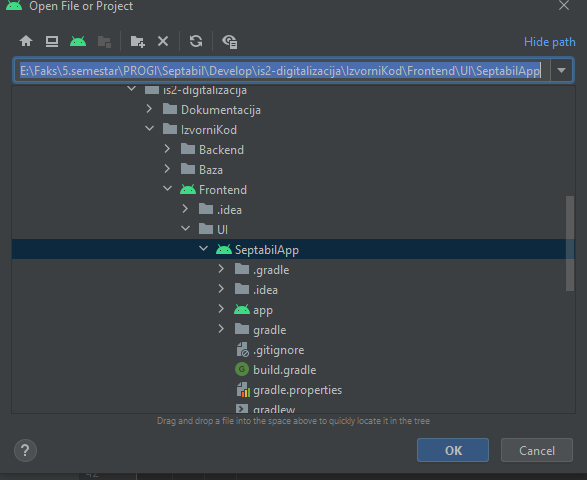
\includegraphics[scale=0.55]{./slike/astudio1.png}
				\caption{Android Studio - Path}
				\label{fig:astudio1}
			\end{figure}
		

			 Nakon što se aplikacija otvori, treba malo pričekati da Gradle učita sve potrebne pakete za rad i onda kada je sve učitano, korisnik treba kliknuti
			 \begin{itemize}
			  \item Build $\rightarrow$ Build Bundle(s) / APK(s) $\rightarrow$ Build APK \end{itemize}
			  kako bi napravio APK naše aplikacije.
			 \begin{figure}[H]
			 	\centering
			 	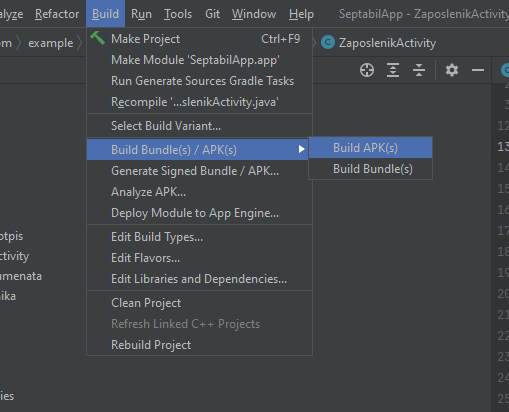
\includegraphics[scale=0.55]{./slike/astudio2.png}
			 	\caption{Android Studio - Build APK}
			 	\label{fig:astudio2}
			 \end{figure} 
			
			
			 \subsection{Postavljanje aplikacije na Amazon App trgovinu}  
			 Za postavljanje aplikacije na Amazon App trgovinu, prvo smo se morali registrirati na Amazon Developer.
			 Nakon toga treba odabrati
			 \begin{itemize}
			 	\item  Apps and Services $\rightarrow$ My apps
			 \end{itemize}
			 kliknuti gumb Add New App, 
			 odabrati želimo li mobilnu ili web aplikaciju i\\ upisati njezino ime.
		 	 \begin{figure}[H]
		 	 	\centering
		 	 	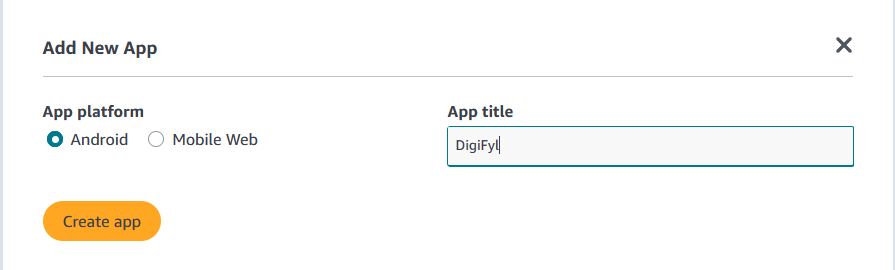
\includegraphics[scale=0.55]{./slike/amzn1.png}
		 	 	\caption{Amazon Developer - Add New App}
		 	 	\label{fig:amzn1}
		 	 \end{figure}
	 	 	\eject
	 	 	Kada odaberemo naziv aplikacije, otvorit će nam se prozor koji ima 6 dijelova za ispuniti, prvi dio su osnovne informacije o aplikaciji poput naslova, kategorije, kontakta...
	 	 	
	 	 	 \begin{figure}[H]
	 	 		\centering
	 	 		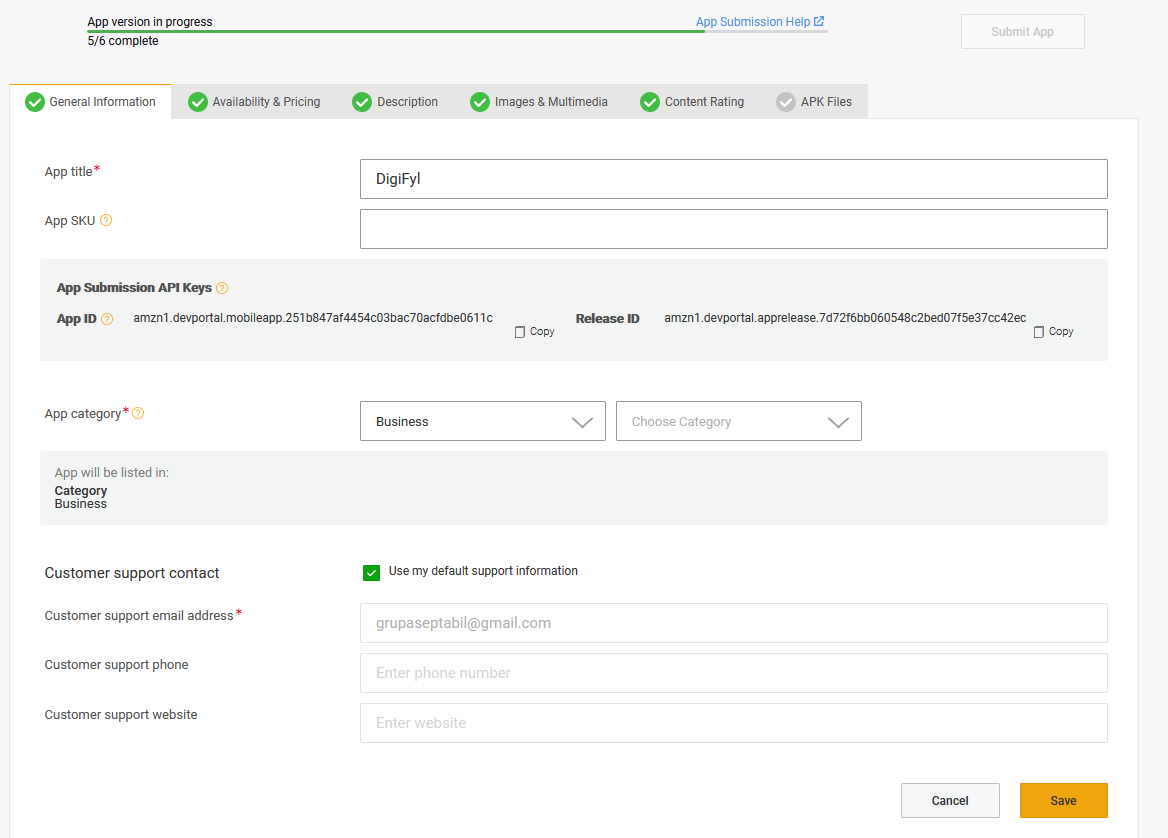
\includegraphics[scale=0.55]{./slike/amzn2.png}
	 	 		\caption{App - General Information}
	 	 		\label{fig:amzn2}
	 	 	\end{figure}
 	 	
 	 	Drugi dio nas samo pita gdje sve želimo da aplikacija bude dostupna u svijetu i želimo li ju izdati kao besplatnu ili naplaćivati.\eject
 	 	Treći dio je opis naše aplikacije, on će biti prikazan kao opis na Amazon App trgovini.
 	 		 \begin{figure}[H]
 	 		\centering
 	 		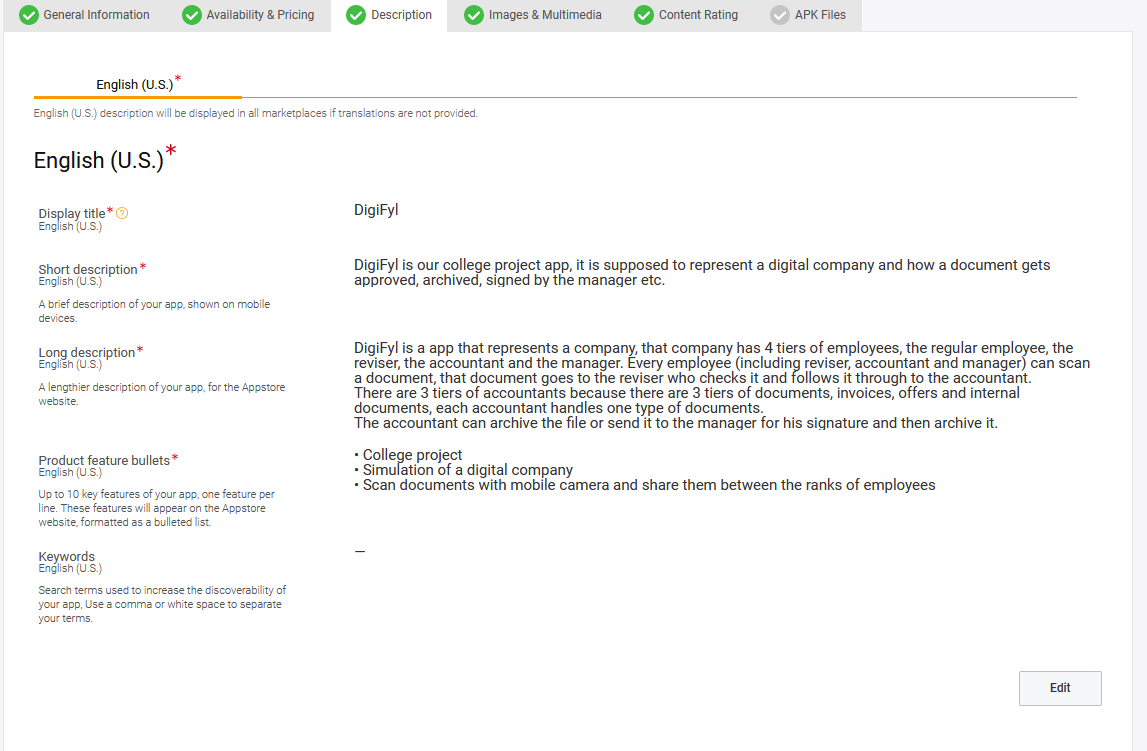
\includegraphics[scale=0.55]{./slike/amzn3.png}
 	 		\caption{App - Description}
 	 		\label{fig:amzn3}
 	 	\end{figure}
  	\eject
  	Četvrti dio od nas traži da postavimo ikonu aplikacije i priložimo 3-10 slika aplikacije, za ikonu smo u ovom slučaju koristili avion koji smo našli na stranici Icon Archive.
  	 \begin{figure}[H]
  		\centering
  		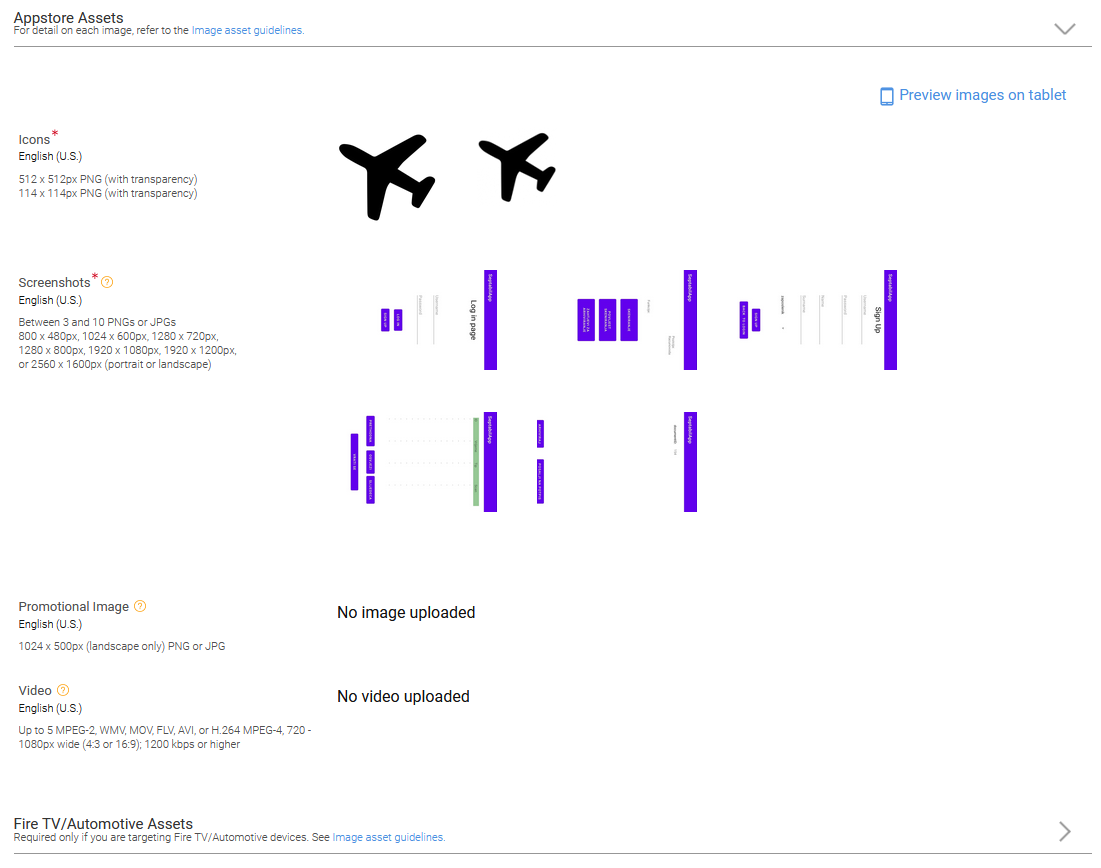
\includegraphics[scale=0.55]{./slike/amzn4.png}
  		\caption{App - Images and multimedia}
  		\label{fig:amzn4}
  	\end{figure} \eject
  
  U petom dijelu moramo napraviti "Content Rating" aplikacije, napisati ima li u njoj nasilja, netolerancije, je li ona u akademske svrhe ili ne...\\ Pita nas i da odaberemo ciljanu publiku te prikuplja li aplikacija osobne podatke. Zadnje stvari koje nas pita je ima li u aplikaciji reklama, kockanja, prikupljamo li lokacije korisnika i ima li komunikacije među korisnicima.\\
  Kako prikupljamo osobne podatke korisnika i oni mogu slati podatke jedni\\ drugima u obliku skeniranog dokumenta, to smo označili s da.
  	 \begin{figure}[H]
  	\centering
  	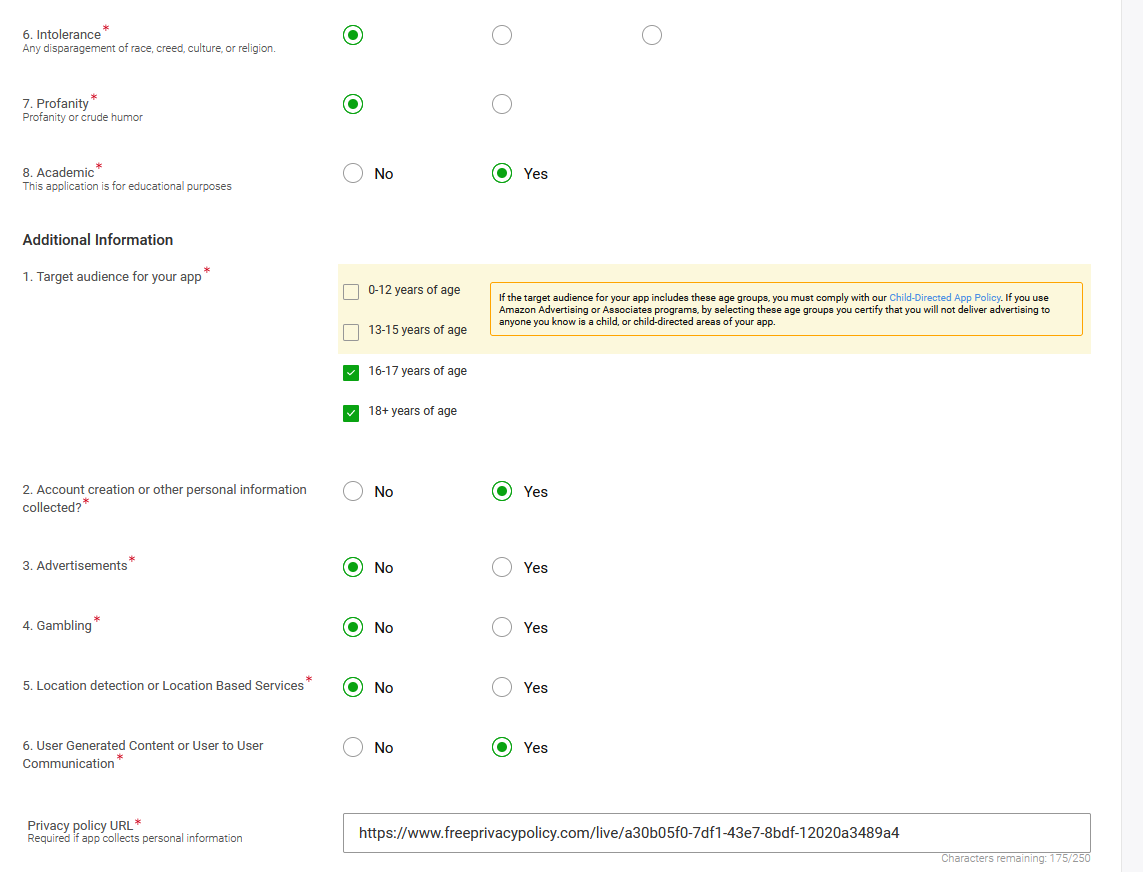
\includegraphics[scale=0.55]{./slike/amzn5.png}
  	\caption{App - Images and multimedia}
  	\label{fig:amzn5}
  \end{figure} 
  Na kraju, s obzirom na to da skupljamo podatke od korisnika, morali smo napraviti politiku privatnosti na kojoj piše koje sve podatke prikupljamo, kako ih koristimo i kako nas se može kontaktirati s bilo kojim dodatnim pitanjima.
  Priložit ćemo ju i ovdje:
  \href{https://www.freeprivacypolicy.com/live/a30b05f0-7df1-43e7-8bdf-12020a3489a4}{\underline{link}}\eject
  	
  	Zadnji dio u deployanju naše aplikacije je odabrati APK datoteku koju\\ predajemo, podržane jezike aplikacije i dodatno napisati upute za testiranje ako će trebati Amazonovom timu, a moramo i odabrati da smo suglasni da se aplikacija uvozi i izvozi iz SAD-a u druge države u kojima Amazon radi.
  		 \begin{figure}[H]
  		\centering
  		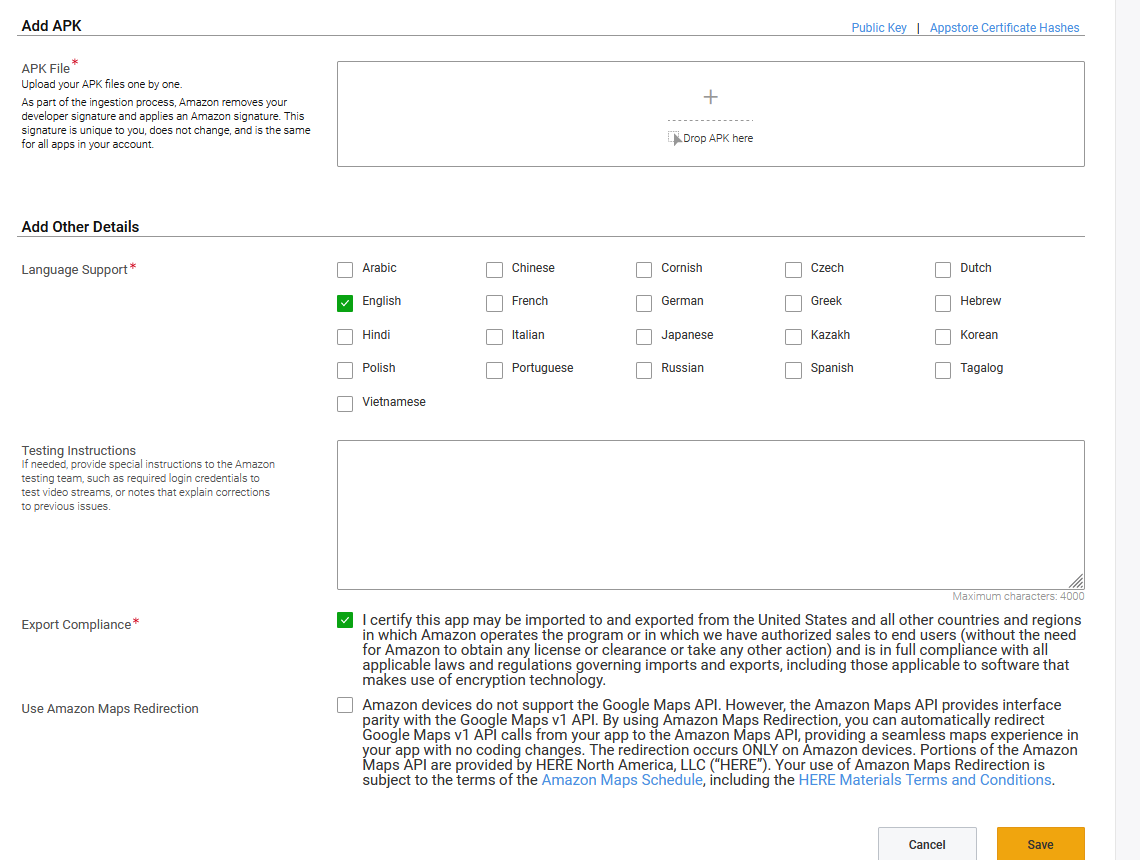
\includegraphics[scale=0.55]{./slike/amzn6.png}
  		\caption{App - APK Files}
  		\label{fig:amzn6}
  	\end{figure} \eject
  
  \subsection{Postavljanje baze podataka na Amazon RDS-u}
 
 Kako bi postavili bazu podataka, morali smo otići na Amazon RDS, odabrati "Databases" i kliknuti "Create Database".\\
 Tad nam se prikaže izbornik koji nas pita za vrstu baze podataka, mi smo radili s postgreSQL bazom.
 	 \begin{figure}[H]
 	\centering
 	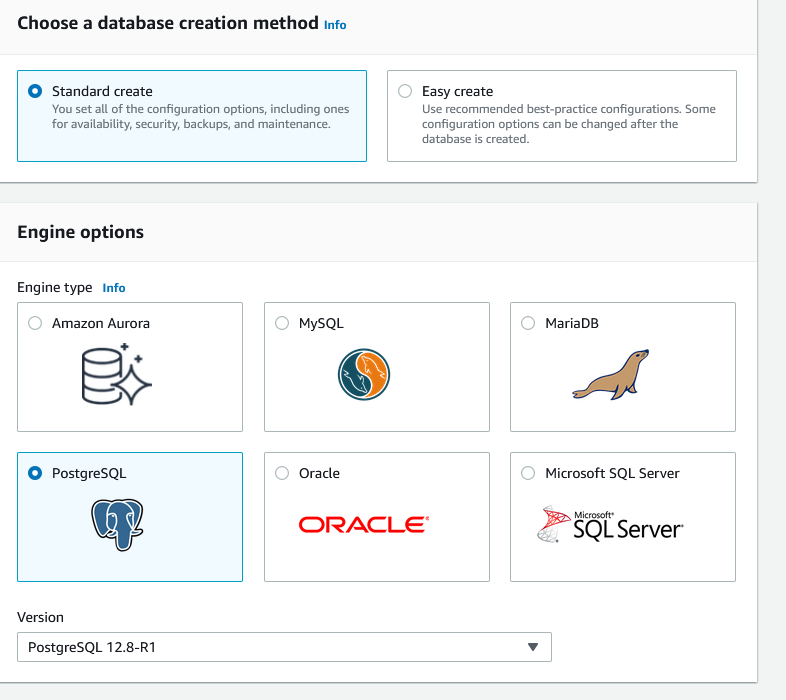
\includegraphics[scale=0.55]{./slike/rds1.png}
 	\caption{Amazon RDS - DB Setup}
 	\label{fig:rds1}
 \end{figure}\eject

Nakon odabira baze podataka, RDS traži da upišemo ime instance baze\\ podataka te da joj priložimo korisničko ime i lozinku kojom će joj se pristupati.
	 \begin{figure}[H]
	\centering
	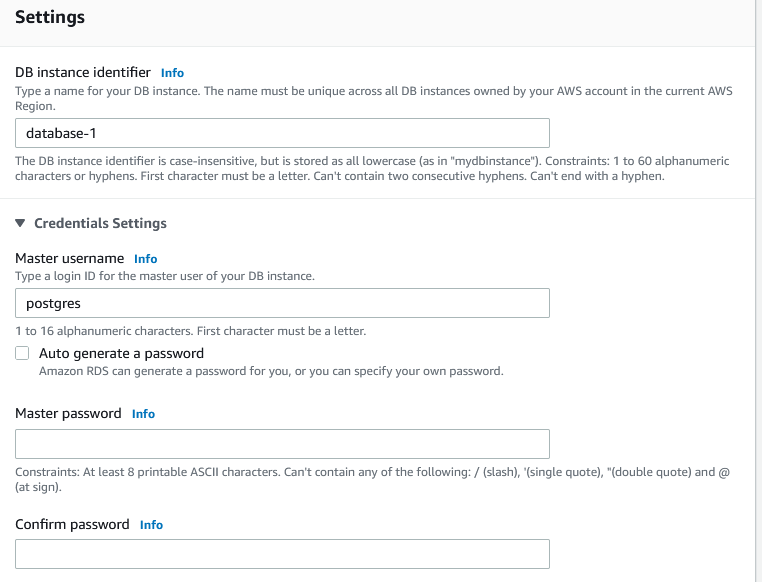
\includegraphics[scale=0.55]{./slike/rds2.png}
	\caption{Amazon RDS - DB Instance}
	\label{fig:rds2}
\end{figure}

Sljedeće što nas RDS pita je koliko nam memorije treba za bazu, minimalan odabir je 20 GB, a nama ni ne treba više pa smo odabrali to, ali smo upalili\\ automatsko skaliranje skladišta, dakle ako nam treba više od 20 GB u nekom\\ trenutku, dobit ćemo tu memoriju.
	 \begin{figure}[H]
	\centering
	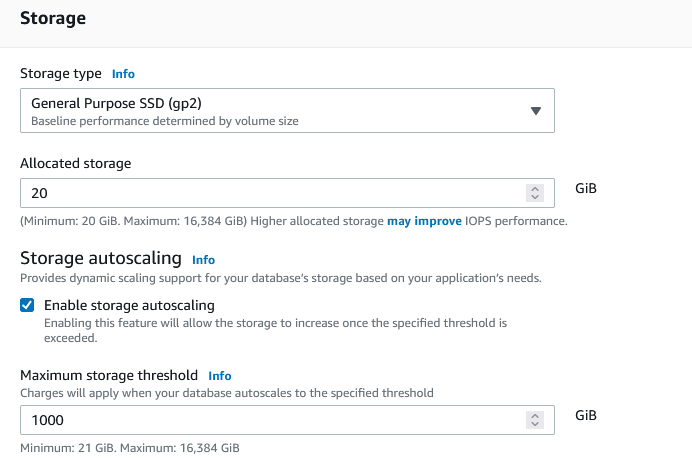
\includegraphics[scale=0.55]{./slike/rds3.png}
	\caption{Amazon RDS - DB Storage}
	\label{fig:rds3}
\end{figure}\eject

Sljedeći obrazac se tiče povezivosti, stvaramo virtualni oblak za našu bazu i grupu podmreža koje baza može koristiti (što smo postavili na sve), također\\ postavljamo i javni pristup našoj bazi kako bi joj mogli pristupiti iz pgAdmin-a.
	 \begin{figure}[H]
	\centering
	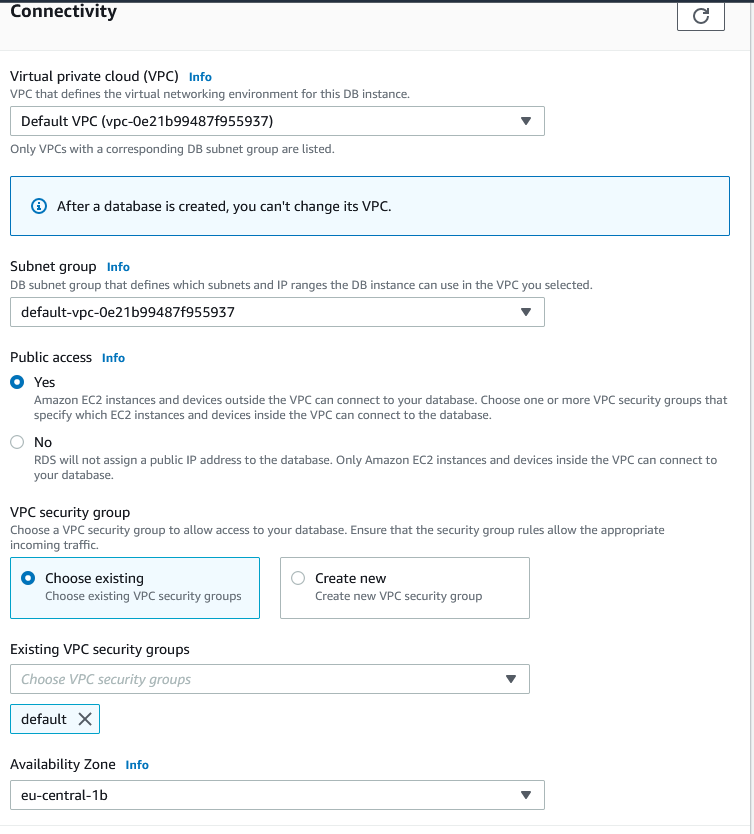
\includegraphics[scale=0.55]{./slike/rds4.png}
	\caption{Amazon RDS - Connectivity}
	\label{fig:rds4}
\end{figure}\eject

Zadnji obrazac nas pita za ime baze podataka i vrijeme zadržavanja sigurnosnih kopija prije brisanja.

	 \begin{figure}[H]
	\centering
	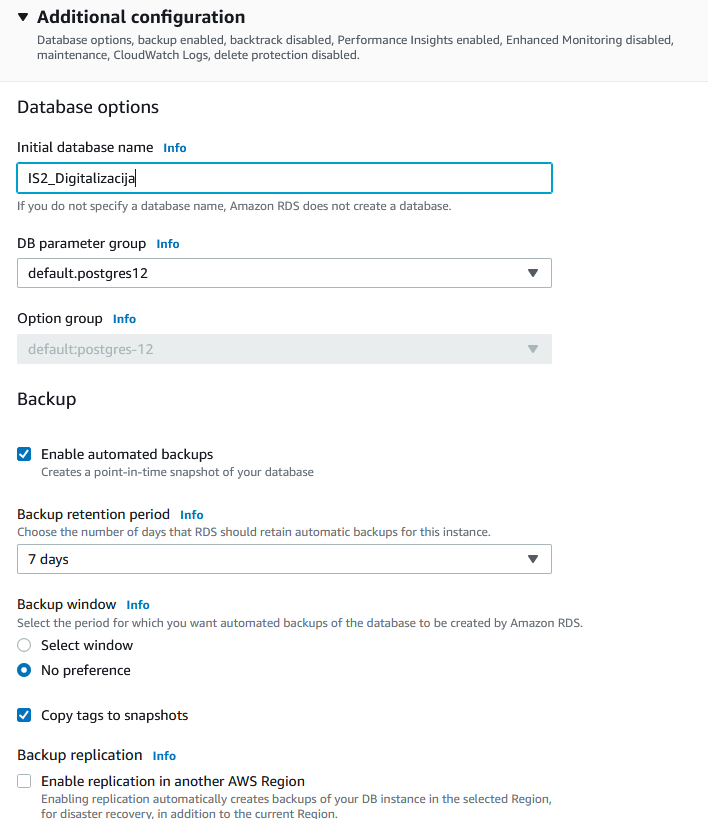
\includegraphics[scale=0.55]{./slike/rds5.png}
	\caption{Amazon RDS - DB Name and Backup}
	\label{fig:rds5}
\end{figure}\eject

Nakon što stvorimo bazu na Amazon RDS-u, dobijemo krajnju točku kako bi se na bazu mogli spojiti iz pgAdmin-a i Python-a. Za spajanje nam trebaju i\\ korisničko ime i lozinka, ali to smo postavili pri stvaranju baze.
	 \begin{figure}[H]
	\centering
	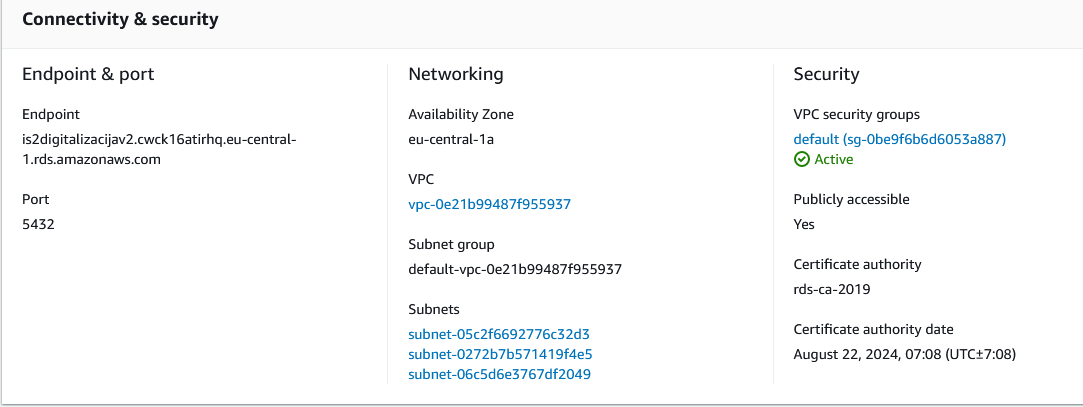
\includegraphics[scale=0.55]{./slike/rds6.png}
	\caption{Amazon RDS - DB Endpoint}
	\label{fig:rds6}
\end{figure}





 
	 	 	 
		 	 
			\eject 
			
	\chapter{Zaključak i budući rad}
		
		
		
		 
		
		
		 
		 Zadatak naše grupe bio je izrada mobilne aplikacije za Android operacijski sustav koja bi ubrzala digitalizaciju računovodstvenim tvrtkama. Izrada aplikacije završena je u zadanom roku, a postupak izrade aplikacije se odvijao u 2 ciklusa.\\
		 \indent U prvom ciklusu nam je cilj bio napraviti jednostavnu verziju aplikacije kako bismo se upoznali s novim tehnologijama i alatima. Nakon okupljanja projektnog tima te nakon upoznavanja sa zadanim zadatkom, krenuli smo prikupljati literaturu te potrebne materijale koji su nam pomogli da se upoznamo s korištenim alatima i tehnologijama. Na prvom sastanku smo se podijelili u manje grupe te je svaka grupa dobila zadatak izrade određenog dijela aplikacije, što nam je uvelike olakšalo izradu same aplikacije. Kroz izradu alfa verzije aplikacije smo se upoznali sa novim alatima i problemima koje smo trebali rješiti, te je alfa verzija aplikacije i dokumentacija bila završena na kraju prvog ciklusa.\\
		 \indent U drugom ciklusu smo implementirali ostale funkcionalnosti aplikacije te ju uredili, reorganizirali bazu podataka i dodali nove lambda funkcije na back-endu. Nakon toga smo napisali i dodali svu potrebnu dokumentaciju.
		  \indent
		 Kroz proces izrade projekta bili smo suočeni s mnogim novim tehnologijama i problemima koji nam prije nisu bili poznati te smo ih sve uspješno rješili i sad smo bogatiji tim znanjem i kompetentniji.
		 Prvo pitanje koje smo rješili je bilo koju čemo infrastrukturu koristiti za izradu projekta, za što je bilo potrebno puno istraživanja raspoloživih opcija te bi rješenje puno brže našli da nam se ponovno postavi isto pitanje, jer smo upoznati sa terenom i opcijama. Isto tako je bilo i sa odabirom alatima koje smo koristili za izradu pojedinih dijelova projekta, kao što su Android studio, AWS-ove lambda funkcije i API gateway, no nakon što smo se upoznali samo je bilo potrebno proniknuti dublje u dostupna znanja alata/ tehnologije kojom se služimo i to sve uspješno povezati u jednu cjelinu sa komunikacijom među svojim dijelovima. Područje znanja koje bi nam nakon ovog projekta najviše pomoglo za kvalitetniji i efikasnije rješen slijedeći projekt je poznavanje Android studia, izrada moblinog dijela aplikacije i front-enda.
		 Nakon ovog projekta smo stekli vrijedno iskustvo izrade potpune aplikacije od početka do kraja sa server-sideom, te bi nam sada izrada nove mobilne aplikacije bila puno jednostavnija i lakša, za što bi se i odlučili da nam se ukaže prilika ili da pronađemo ideju vrijednu realizacije.
		  \indent
		 Funkcionalnosti koje bi još ostvarili da usavršavamo aplikaciju bi bilo dodavanje pop-up obavijesti naše aplikacije.
		 
		
		\eject 
	\chapter*{Popis literature}
		\addcontentsline{toc}{chapter}{Popis literature}
	 	
 		\textbf{\textit{Kontinuirano osvježavanje}}
	
		\textit{Popisati sve reference i literaturu koja je pomogla pri ostvarivanju projekta.}
		
		
		\begin{enumerate}
			
			
			\item  Programsko inženjerstvo, FER ZEMRIS, \url{http://www.fer.hr/predmet/proinz}
			
			\item  I. Sommerville, "Software engineering", 8th ed, Addison Wesley, 2007.
			
			\item  T.C.Lethbridge, R.Langaniere, "Object-Oriented Software Engineering", 2nd ed. McGraw-Hill, 2005.
			
			\item  I. Marsic, Software engineering book``, Department of Electrical and Computer Engineering, Rutgers University, \url{http://www.ece.rutgers.edu/~marsic/books/SE}
			
			\item  The Unified Modeling Language, \url{https://www.uml-diagrams.org/}
			
			\item  Astah Community, \url{http://astah.net/editions/uml-new}
		\end{enumerate}
		
		 
	
	
	\begingroup
	\renewcommand*\listfigurename{Indeks slika i dijagrama}
	%\renewcommand*\listtablename{Indeks tablica}
	%\let\clearpage\relax
	\listoffigures
	%\vspace{10mm}
	%\listoftables
	\endgroup
	\addcontentsline{toc}{chapter}{Indeks slika i dijagrama}


	
	\eject 
		
	\chapter*{Dodatak: Prikaz aktivnosti grupe}
		\addcontentsline{toc}{chapter}{Dodatak: Prikaz aktivnosti grupe}
		
		\section*{Dnevnik sastajanja}
		
		\textbf{\textit{Kontinuirano osvježavanje}}\\
		
	
		
		\begin{packed_enum}
			\item  sastanak
			
			\item[] \begin{packed_item}
				\item Datum: u ovom formatu: 19.10.2021
				\item Prisustvovali: Cijeli tim
				\item Teme sastanka:
				\begin{packed_item}
					\item  analiza zadatka
					\item  prva slika arhitekture sustava
					\item  generalna podjela posla
				\end{packed_item}
			\end{packed_item}
			
			\item  sastanak
			\item[] \begin{packed_item}
				\item Datum: u ovom formatu: 7.11.2021
				\item Prisustvovali: Cijeli tim
				\item Teme sastanka:
				\begin{packed_item}
					\item  detaljnija razrada arhitekture
					\item  rasprava o detaljima implementacije

				\end{packed_item}
			\end{packed_item}
		
		
		\item  sastanak
		\item[] \begin{packed_item}
			\item Datum: u ovom formatu: 9.11.2021
			\item Prisustvovali: Cijeli tim
			\item Teme sastanka:
			\begin{packed_item}
				\item  konačna razrada arhitekture
			\end{packed_item}
		\end{packed_item}
	
	\item  sastanak
	\item[] \begin{packed_item}
		\item Datum: u ovom formatu: 16.11.2021
		\item Prisustvovali: Cijeli tim
		\item Teme sastanka:
		\begin{packed_item}
			\item  raspodjela pisanja dokumentacije
		\end{packed_item}
	\end{packed_item}

	\item  sastanak
	\item[] \begin{packed_item}
		\item Datum: u ovom formatu: 13.12.2021
		\item Prisustvovali: Cijeli tim
		\item Teme sastanka:
		\begin{packed_item}
			\item  plan alfa verzije i gruba raspodjela ostatka posla pri kreiranju iste
		\end{packed_item}
	\end{packed_item}
	

			
			%
			
		\end{packed_enum}
		
		\eject
		\section*{Tablica aktivnosti}
		
			\textbf{\textit{Kontinuirano osvježavanje}}\\
			
			 \textit{Napomena: Doprinose u aktivnostima treba navesti u satima po članovima grupe po aktivnosti.}

			\begin{longtblr}[
					label=none,
				]{
					vlines,hlines,
					width = \textwidth,
					colspec={X[7, l]X[1, c]X[1, c]X[1, c]X[1, c]X[1, c]X[1, c]X[1, c]}, 
					vline{1} = {1}{text=\clap{}},
					hline{1} = {1}{text=\clap{}},
					rowhead = 1,
				} 
				\multicolumn{1}{c|}{} & \multicolumn{1}{c|}{\rotatebox{90}{\textbf{Dominik Jurinčić}}} & \multicolumn{1}{c|}{\rotatebox{90}{\textbf{Marko Bunić }}} &	\multicolumn{1}{c|}{\rotatebox{90}{\textbf{Marko Husnjak }}} & \multicolumn{1}{c|}{\rotatebox{90}{\textbf{Jakov Prister }}} &	\multicolumn{1}{c|}{\rotatebox{90}{\textbf{Filip Martinović }}} & \multicolumn{1}{c|}{\rotatebox{90}{\textbf{Borna Radojčić }}} &	\multicolumn{1}{c|}{\rotatebox{90}{\textbf{Ivan Lovrić }}} \\  
				Upravljanje projektom 		&2  &2  &1  &  &  &  & \\ 
				Opis projektnog zadatka 	&  &7  &1  &  &  & \\ 
				
				Funkcionalni zahtjevi       &  &  &3  &  &  &  &  \\ 
				Opis pojedinih obrazaca 	&  &  &  &  &4  &  &  \\ 
				Dijagram obrazaca 			&  &  &  &  & 7 &  &  \\ 
				Sekvencijski dijagrami 		&  &  &  &4  &  &  &  \\ 
				Opis ostalih zahtjeva 		&  &  &  &  &  &1  &1  \\ 

				Arhitektura i dizajn sustava	 &2  &  &3  &  &  &  &  \\ 
				Baza podataka				&  &  &  &  &  &1  &1   \\ 
				Dijagram razreda 			&  &  &  &  &4  &  &   \\ 
				Dijagram stanja				&  &2  &  &  &  &  &  \\ 
				Dijagram aktivnosti 		&  &  &  &2  &  &  &  \\ 
				Dijagram komponenti			&  &  &  &  &  &  &4  \\ 
				Korištene tehnologije i alati 		&1  &  &1  &  &  &  &  \\ 
				Ispitivanje programskog rješenja 	&4  &  &1  &  &6  &6  &  \\ 
				Dijagram razmještaja			&  &  &  &3  &  &  &  \\ 
				Upute za puštanje u pogon 		&  &  &  &  &  &5  &  \\  
				Dnevnik sastajanja 			&1  &  &  &  &  &1  &  \\ 
				Zaključak i budući rad 		&  &1  &  &  &  &  &1  \\  
				Popis literature 			&  &  &  &  &  &  &  \\  
				&  &  &  &  &  &  &  \\ \hline 
				\textit{Dodatne stavke kako ste podijelili izradu aplikacije -- ostavio sam da navedete svoje dijelove -M.B.} 			&  &  &  &  &  &  &  \\ 
				\textit{izrada UI-a i front-end aplikacije} 				&  &5  &18  &10  &3  &  &  \\  
				\textit{izrada baze podataka} 		 			&  &  &  &  &  &17  &17 \\  

				\textit{spajanje back-enda s bazom podataka} 							&3  &  &  &4  &  &4  &4  \\ 
				\textit{rad na back-end-u i lambda funkcijama} 							&10  &  &  &2  &  &  &  \\  
				 							 
				\textit{spajanje s bazom podataka} 							&8  &  &  &4  &  &4  &4  \\ 
				\textit{back end} 							&12  &  &  &2  &  &  &  \\  
				 							 
				\textit{Povezivanje front-enda i back-enda} 							&2  &2  &2  &  &  &  &  \\ 
 
				 						
				\textit{Ispitivanje AWS i ostalih usluga za rješenje infrastukture} 							&4  &4  &1  &4  &  &4  &4  \\ 
				\textit{Istraživanje prikladnog rješenja arhitekture} 							&3  &8  &1  &  &  &  &  \\
				\textit{implementacija ugrađene kamere,slikanja, OCR-a i akcelerometra} 
				&  &  &  &  & 15 &  &\
			\end{longtblr}
					
					
		\eject
		\section*{Dijagrami pregleda promjena}
		
		\begin{figure}[H]
			\centering
			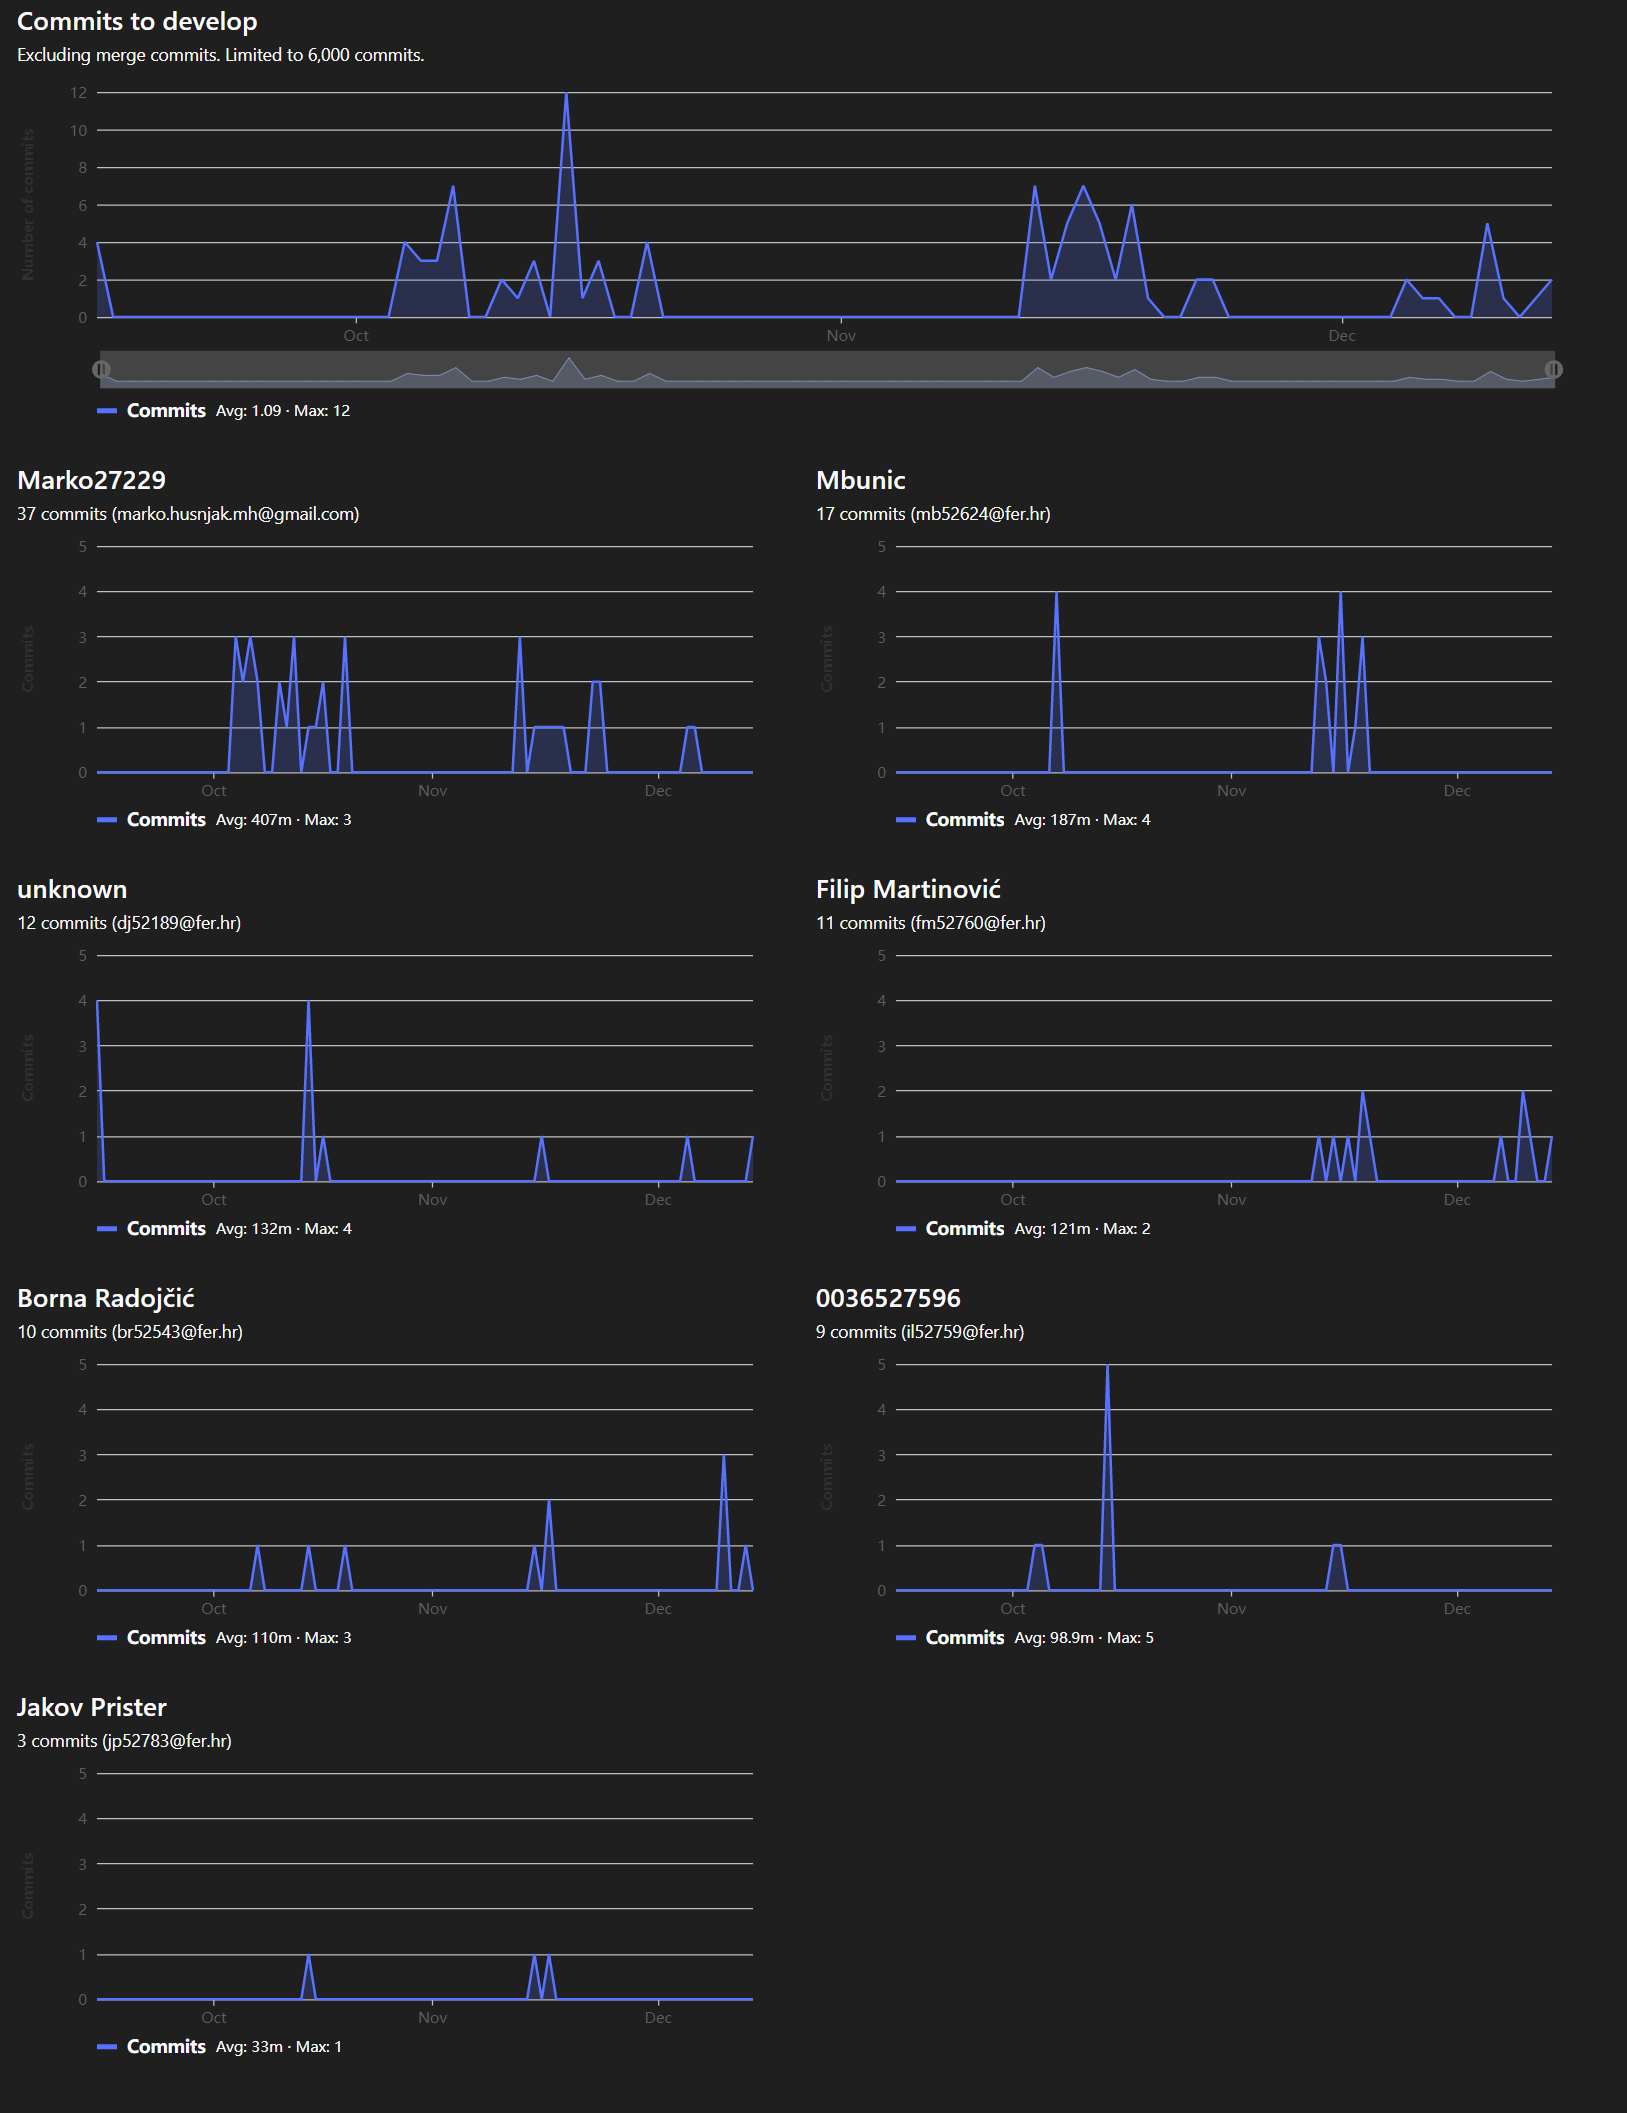
\includegraphics[scale=0.5]{./slike/develop.png}
			\caption{"Dijagram develop"}
			\label{fig:develop}
		\end{figure}
	
		\begin{figure}[H]
			\centering
			\includegraphics[scale=0.5]{./slike/devdoc.png}
			\caption{"Dijagram devdoc"}
			\label{fig:devdoc}
		\end{figure}
		
	


\end{document} %naredbe i tekst nakon ove naredbe ne ulaze u izgrađen dokument 


